\documentclass[10pt,a4paper]{article}

\usepackage[top=1.6cm,bottom=1.6cm,left=1.75cm,right=1.75cm]{geometry}
\usepackage{graphicx}
\usepackage{amsmath}
\usepackage{booktabs}
\usepackage{subcaption}
\usepackage{siunitx}
\usepackage{placeins}
\usepackage[hidelinks]{hyperref}

% figures come from media/ and scripts and outputs/tier_1/output/
\graphicspath{{../../media/}{../../scripts and outputs/tier_1/output/}}
\setlength{\textfloatsep}{10pt plus 2pt minus 2pt}
\setlength{\floatsep}{8pt plus 2pt minus 2pt}
\setlength{\intextsep}{8pt plus 2pt minus 2pt}
\renewcommand{\topfraction}{0.9}\renewcommand{\bottomfraction}{0.8}\renewcommand{\textfraction}{0.1}\renewcommand{\floatpagefraction}{0.8}

\newcommand{\repo}{https://github.com/Shass27/curiosity-perseverance-wheel-fea}
\newcommand{\tree}{\repo/tree/main}
\newcommand{\blob}{\repo/blob/main}

\title{Curiosity Rover Wheel Failure Analysis}
\author{Pabitra Kumar Sahoo \and Ridam Bagul \and Sibasis Panda \and Shaswath S}
\date{}

\begin{document}
\maketitle

\begin{abstract}
\noindent The thin aluminium skin of the Curiosity rover's wheels has cracked in service, mostly where the skin meets the stiff ridges (grousers) that give the wheel its grip. This report asks why. We study a small flat piece of skin between two grousers, pressed by a rock of varying sharpness, and estimate the stress in it in two ways: a quick hand calculation that treats the skin as a clamped beam, and detailed computer simulations (finite element analysis, FEA) in Ansys. Because simulation results depend on how finely the model is divided up, each case was run on three levels of detail (element sizes of 10, 1 and \SI{0.1}{mm}). The coarsest model gives badly wrong, even inconsistent, answers; the two finer ones agree closely, so the finest is used for all conclusions. The results show that the stress at the skin--grouser junction exceeds the material's fatigue limit (\SI{106}{MPa}) for every rock size tested, and the stress directly under the rock does so for sharp rocks. The hand calculation captures the overall pattern but under-predicts the stress under sharp rocks and over-predicts it at the junction, so it is a useful first guide, not a final design check.
\end{abstract}

% ---------------------------------------------------------------
\section{Introduction}

NASA and JPL mission reports have documented punctures and cracks in the wheels of the Curiosity rover after driving over angular, embedded rocks~\cite{nasa}. The wheel skin is a thin aluminium shell stiffened by chevron-shaped grousers. A rock pressing on the skin between two grousers bends the skin like a plate clamped along its stiffened edges. The bending moment, and hence the surface stress, is largest at two places: directly under the rock, and at the skin--grouser junction, where the section changes abruptly and a small fillet concentrates the stress.

This report asks a narrow question: \emph{for a given rock sharpness, how large are the junction and centre stresses, and can a hand calculation predict them?} The region studied is marked in Figure~\ref{fig:location}(a). It is idealised as the flat segment shown in Figure~\ref{fig:location}(b), and the patch radius $a$ stands in for rock sharpness: a smaller $a$ is a sharper rock. Because a hand calculation is only as useful as the reference it is checked against, the report also asks whether the FEA itself is mesh-independent, and repeats the comparison on three progressively finer meshes. All CAD, data and scripts are in the project repository~\cite{repo}, and the report links to them rather than reproducing them.

\begin{figure}[htbp]
  \centering
  \begin{subfigure}[b]{0.38\textwidth}
    \centering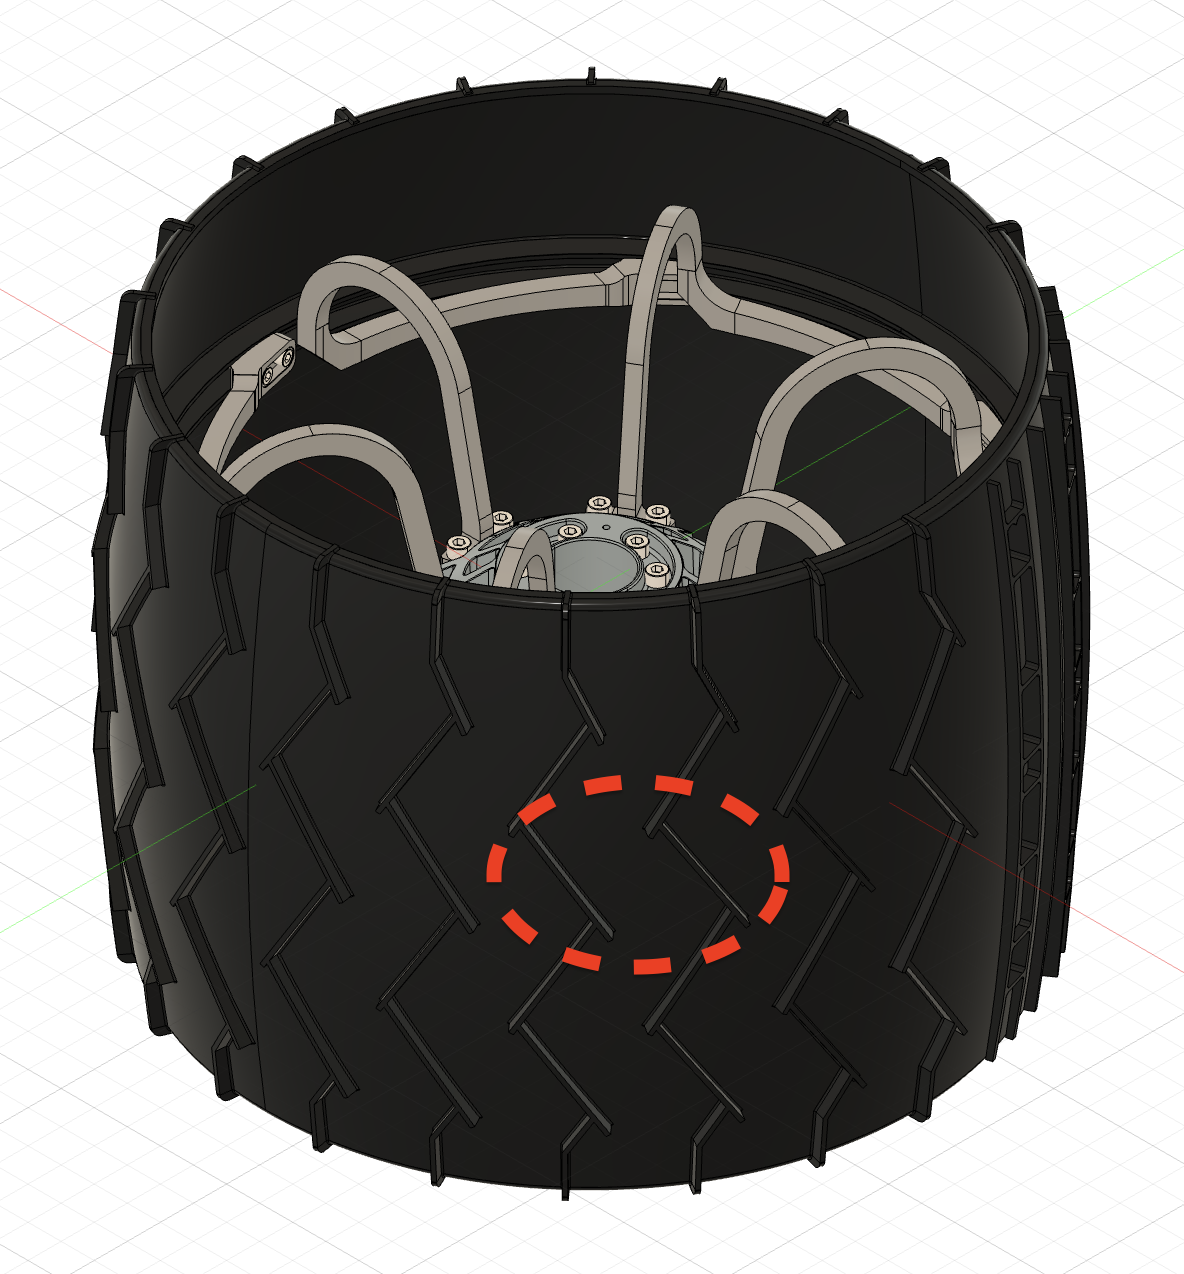
\includegraphics[width=\linewidth]{analysis_location.png}
    \caption{Region of the wheel analysed}
  \end{subfigure}\hfill
  \begin{subfigure}[b]{0.55\textwidth}
    \centering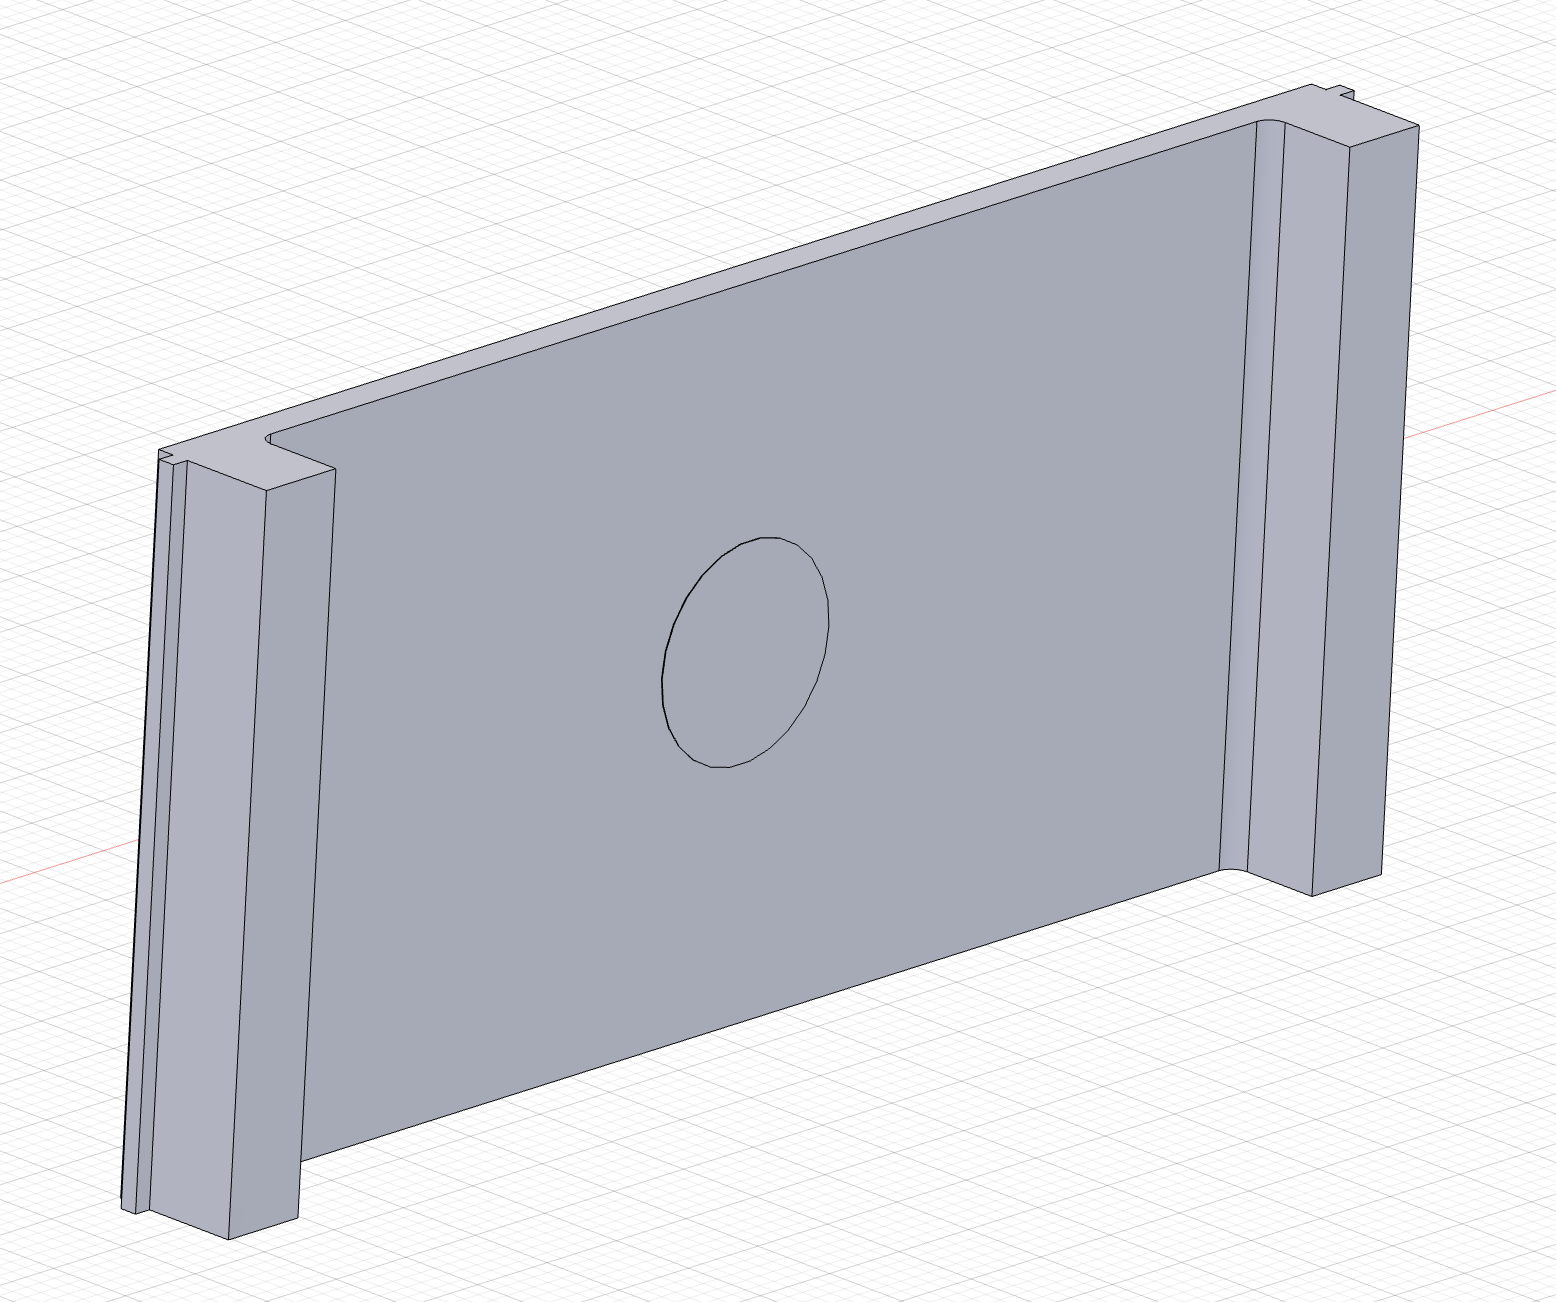
\includegraphics[width=\linewidth]{analysis_segment.png}
    \caption{Idealised skin segment with load patch}
  \end{subfigure}
  \caption{Location of the analysed segment on the wheel and the CAD model used.}
  \label{fig:location}
\end{figure}

% ---------------------------------------------------------------
\section{Model and FEA setup}

The segment is a \SI{2}{mm} skin between two grouser blocks, each \SI{5}{mm} wide and \SI{7.5}{mm} deep overall. The skin meets each block through an R\SI{1}{mm} fillet (Table~\ref{tab:inputs}). The two outer end faces are fixed, which represents the continuation of the wheel shell beyond the grousers. The load is a uniform pressure on a circular patch at mid-span, with $a = 2, 4, 6, 8, \SI{10}{mm}$. One \href{\tree/CAD_models/Tier\%201}{CAD file per radius} carries the patch as a split face.

The FEA was solved in Ansys Mechanical 2025 R1 with solid elements at a total force of \SI{300}{N}. Stress was extracted as a \emph{linearized equivalent stress} along a straight path \SI{2}{mm} above the base, which is the top surface of the skin, running across the full \SI{85}{mm} span (Figure~\ref{fig:ansys}). Ansys splits the stress along a path into membrane, bending and peak parts~\cite{ansys}. This report uses the \emph{Total} column, which is the actual von Mises stress at each path point. The analysis load is a design choice of \SI{400}{N}. The model is linear-elastic, so the FEA values are scaled by $400/300$ before any comparison. The \href{\tree/Simulation\%20results/Tier\%201}{exported path data} is in the repository.

Each of the five load cases was solved on three meshes, labelled by their nominal element size: \SI{10}{mm}, \SI{1}{mm} and \SI{0.1}{mm}. For scale, the skin is \SI{2}{mm} thick and the fillet radius is \SI{1}{mm}, so a \SI{10}{mm} element is five times the skin thickness, a \SI{1}{mm} element is the size of the fillet radius, and a \SI{0.1}{mm} element is one twentieth of the skin thickness. The geometry, load, constraints and the path (the same 85\,mm path, sampled every \SI{1.77}{mm}) are identical in all three runs, so any difference between them is due to the mesh alone.

\begin{table}[htbp]
  \centering
  \caption{Model inputs.}
  \label{tab:inputs}
  \begin{tabular}{llr}
    \toprule
    Quantity & Symbol & Value \\
    \midrule
    Skin thickness & $t$ & \SI{2}{mm} \\
    Grouser depth / width & $D$, $w_g$ & \SI{7.5}{mm}, \SI{5}{mm} \\
    Overall length (fixed ends) & $L$ & \SI{83}{mm} \\
    Panel width & $b$ & \SI{40}{mm} \\
    Junction fillet radius & $r$ & \SI{1}{mm} \\
    Total load & $P$ & \SI{400}{N} (FEA at \SI{300}{N}, scaled) \\
    Patch radius & $a$ & 2--\SI{10}{mm} \\
    Mesh (nominal element size) & -- & 10, 1, \SI{0.1}{mm} \\
    Material & -- & Al 7075-T7351, $E = \SI{72}{GPa}$, $\nu = 0.33$ \\
    Fatigue limit & $\sigma_f$ & \SI{106}{MPa} \\
    \bottomrule
  \end{tabular}
\end{table}

\begin{figure}[htbp]
  \centering
  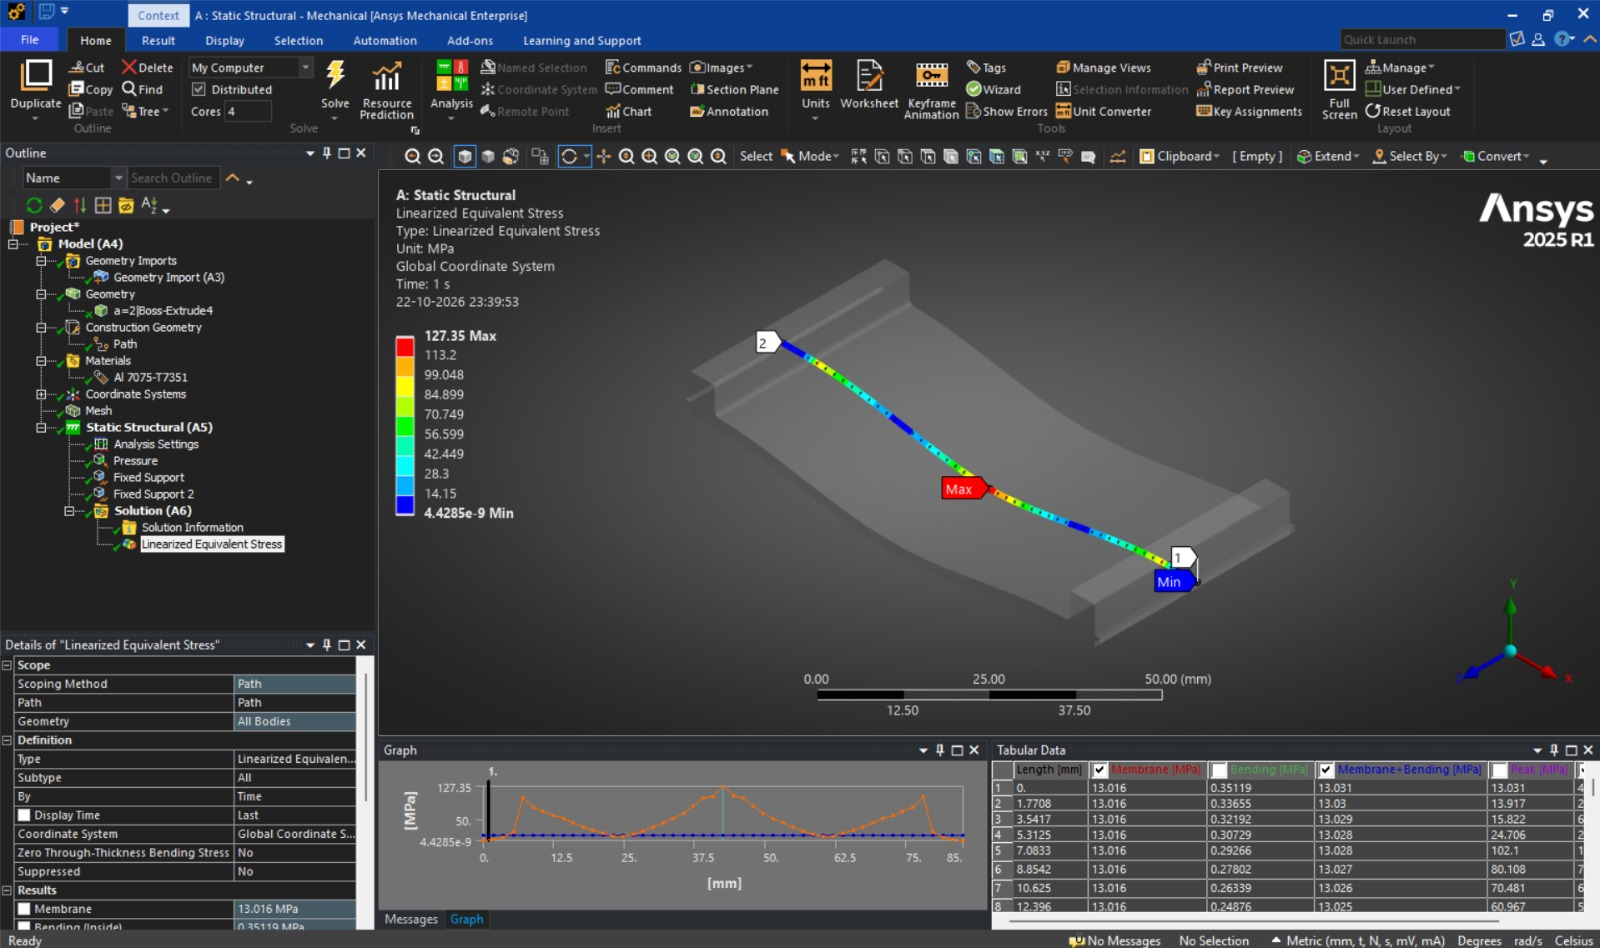
\includegraphics[width=0.85\textwidth]{fea run ex1 tier1.jpeg}
  \caption{Ansys 2025 R1 run for $a = \SI{2}{mm}$ at \SI{300}{N}: the linearized equivalent stress path on the skin, with the stress plotted along the path and the tabular output.}
  \label{fig:ansys}
\end{figure}

% ---------------------------------------------------------------
\section{Analytical model}

The model follows classical beam and plate theory in the form tabulated by Roark. It is implemented in \href{\blob/scripts\%20and\%20outputs/tier_1/path_stress_analytical.m}{\texttt{path\_stress\_analytical.m}}, and the results are compared in \href{\blob/scripts\%20and\%20outputs/tier_1/fea_vs_analytical.m}{\texttt{fea\_vs\_analytical.m}}.

\subsection{Patch load}
A uniform pressure $P/\pi a^2$ on a circle of radius $a$, integrated across the width, gives a line load along the span $x$:
\begin{equation}
  q(x) = \frac{P}{\pi a^2}\, 2\sqrt{a^2 - (x - x_c)^2}, \qquad |x - x_c| \le a,
\end{equation}
which integrates to $P$. Here $x_c = L/2$ is the patch centre.

\subsection{Fixed stepped beam}
The segment is treated as a beam of width $b$, fixed at $x = 0$ and $x = L$. Its second moment of area $I(x)$ is $bD^3/12$ inside the grouser blocks and $bt^3/12$ over the skin. With $M_q(x)$ the moment of the load to the left of $x$,
\begin{equation}
  M(x) = M_0 + V_0 x - M_q(x),
\end{equation}
and the two unknown end reactions follow from zero slope and zero deflection at the far clamp:
\begin{equation}
  \int_0^L \frac{M}{EI}\,dx = 0, \qquad \int_0^L \frac{M\,(L - x)}{EI}\,dx = 0 .
\end{equation}
This handles the stepped section and any load shape without tables. As $a \to 0$ with rigid grousers it recovers the textbook result $|M| = PL'/8$ at both the ends and the centre of the clear span $L'$. The script checks this limit on every run.

\subsection{Stress on the path}
On the skin surface the bending stress is $\sigma_x = 6M/(bt^2)$, the nominal stress $\sigma_\text{nom}$. At the junction the fillet raises it to
\begin{equation}
  \sigma_\text{max} = K_t\, \sigma_\text{nom},
\end{equation}
where $K_t$ is taken from Peterson's fit for a stepped flat bar with a shoulder fillet in bending. With $h/r = 2.75$ and $2h/D = 0.73$, this gives $K_t = 1.63$. The top surface is traction-free ($\sigma_z = 0$), and a wide plate in cylindrical bending is restrained laterally, so $\sigma_y = \nu\sigma_x$. The principal stresses are then $(\sigma_x, \nu\sigma_x, 0)$, and the von Mises stress is
\begin{equation}
  \sigma_\text{vm} = |\sigma_x|\sqrt{1 - \nu + \nu^2}.
\end{equation}

% ---------------------------------------------------------------
\section{Results}

\subsection{Analytical}
The analytical stress along the path (Figure~\ref{fig:analytical}a) is piecewise linear, as beam theory requires. It peaks at both junctions and under the patch, and passes through zero at the two inflection points near the quarter-spans. Patch size changes only the centre peak, because spreading the load flattens the moment under it, while the junction moment is almost insensitive to $a$ (Table~\ref{tab:summary}). The nominal junction stress (von Mises, without $K_t$) is about \SI{120}{MPa}, which becomes about \SI{195}{MPa} once $K_t$ is applied. Both values exceed the fatigue limit, as do the centre stresses for $a \le \SI{4}{mm}$; at $a = \SI{6}{mm}$ the centre stress (\SI{105.1}{MPa}) is just below it.

\begin{figure}[htbp]
  \centering
  \begin{subfigure}[b]{0.43\textwidth}
    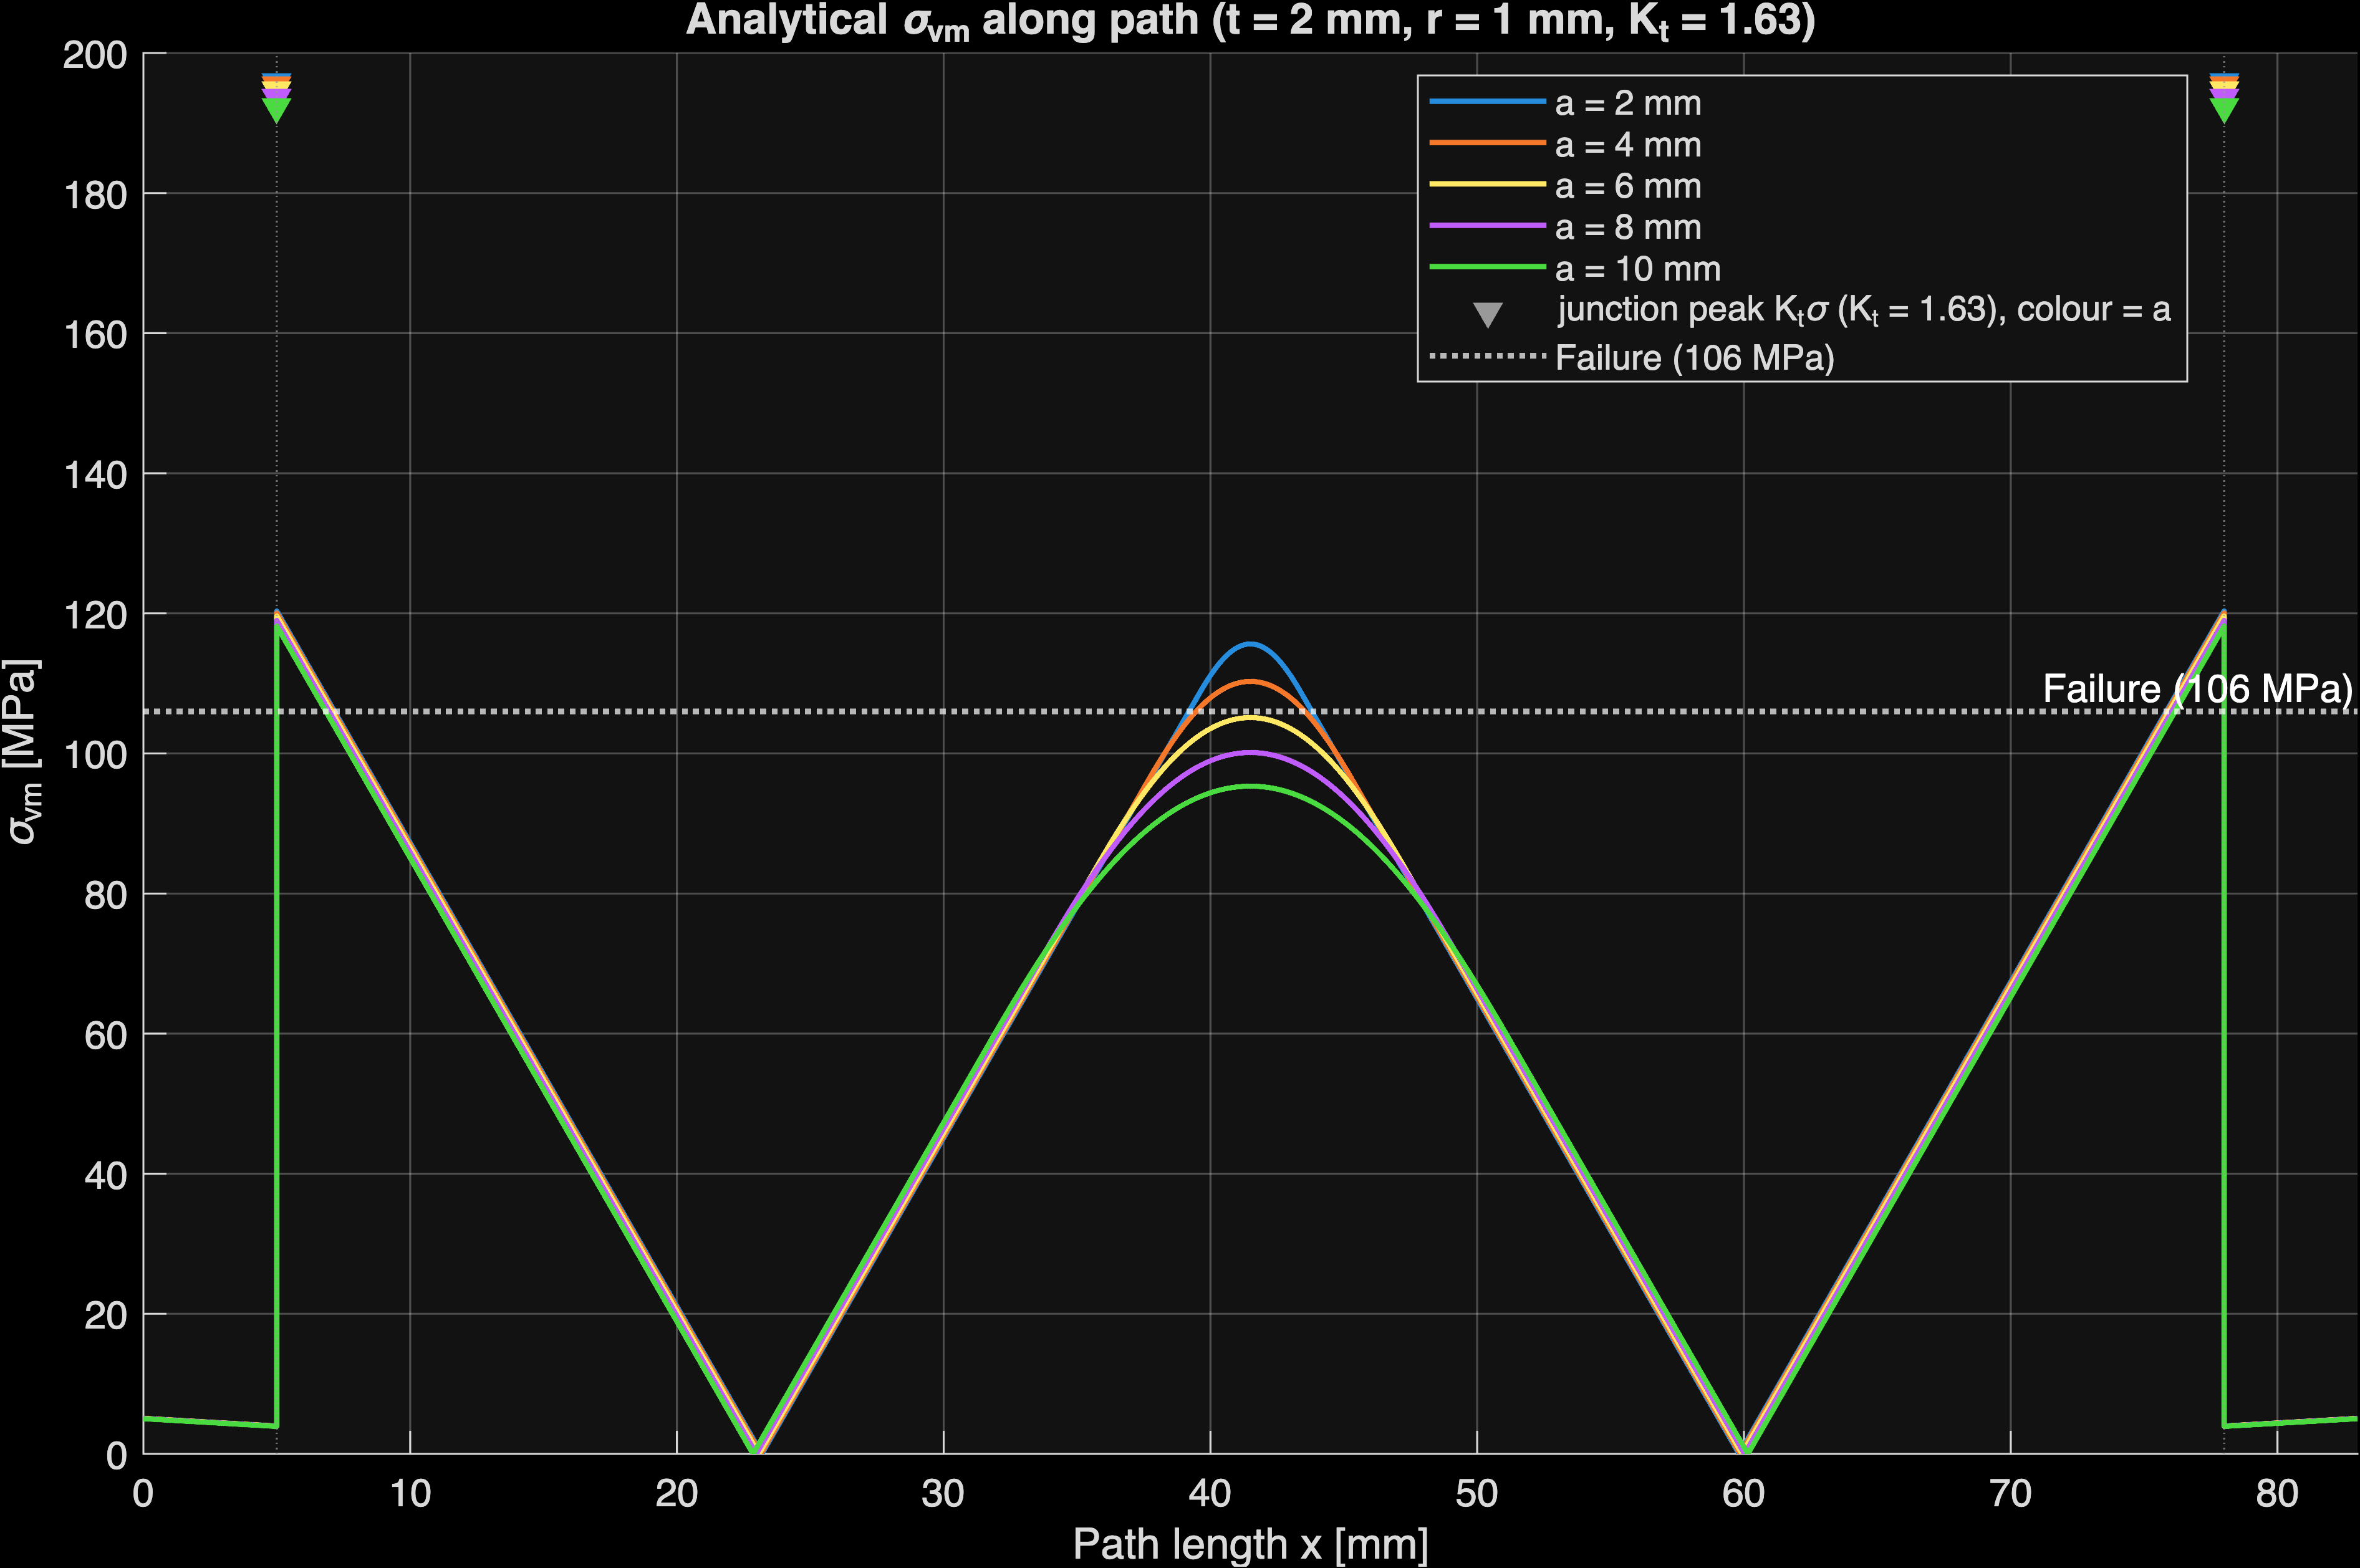
\includegraphics[width=\linewidth]{analytical_path_stress_vs_x.png}
    \caption{$\sigma_\text{vm}$ along the path}
  \end{subfigure}\hfill
  \begin{subfigure}[b]{0.43\textwidth}
    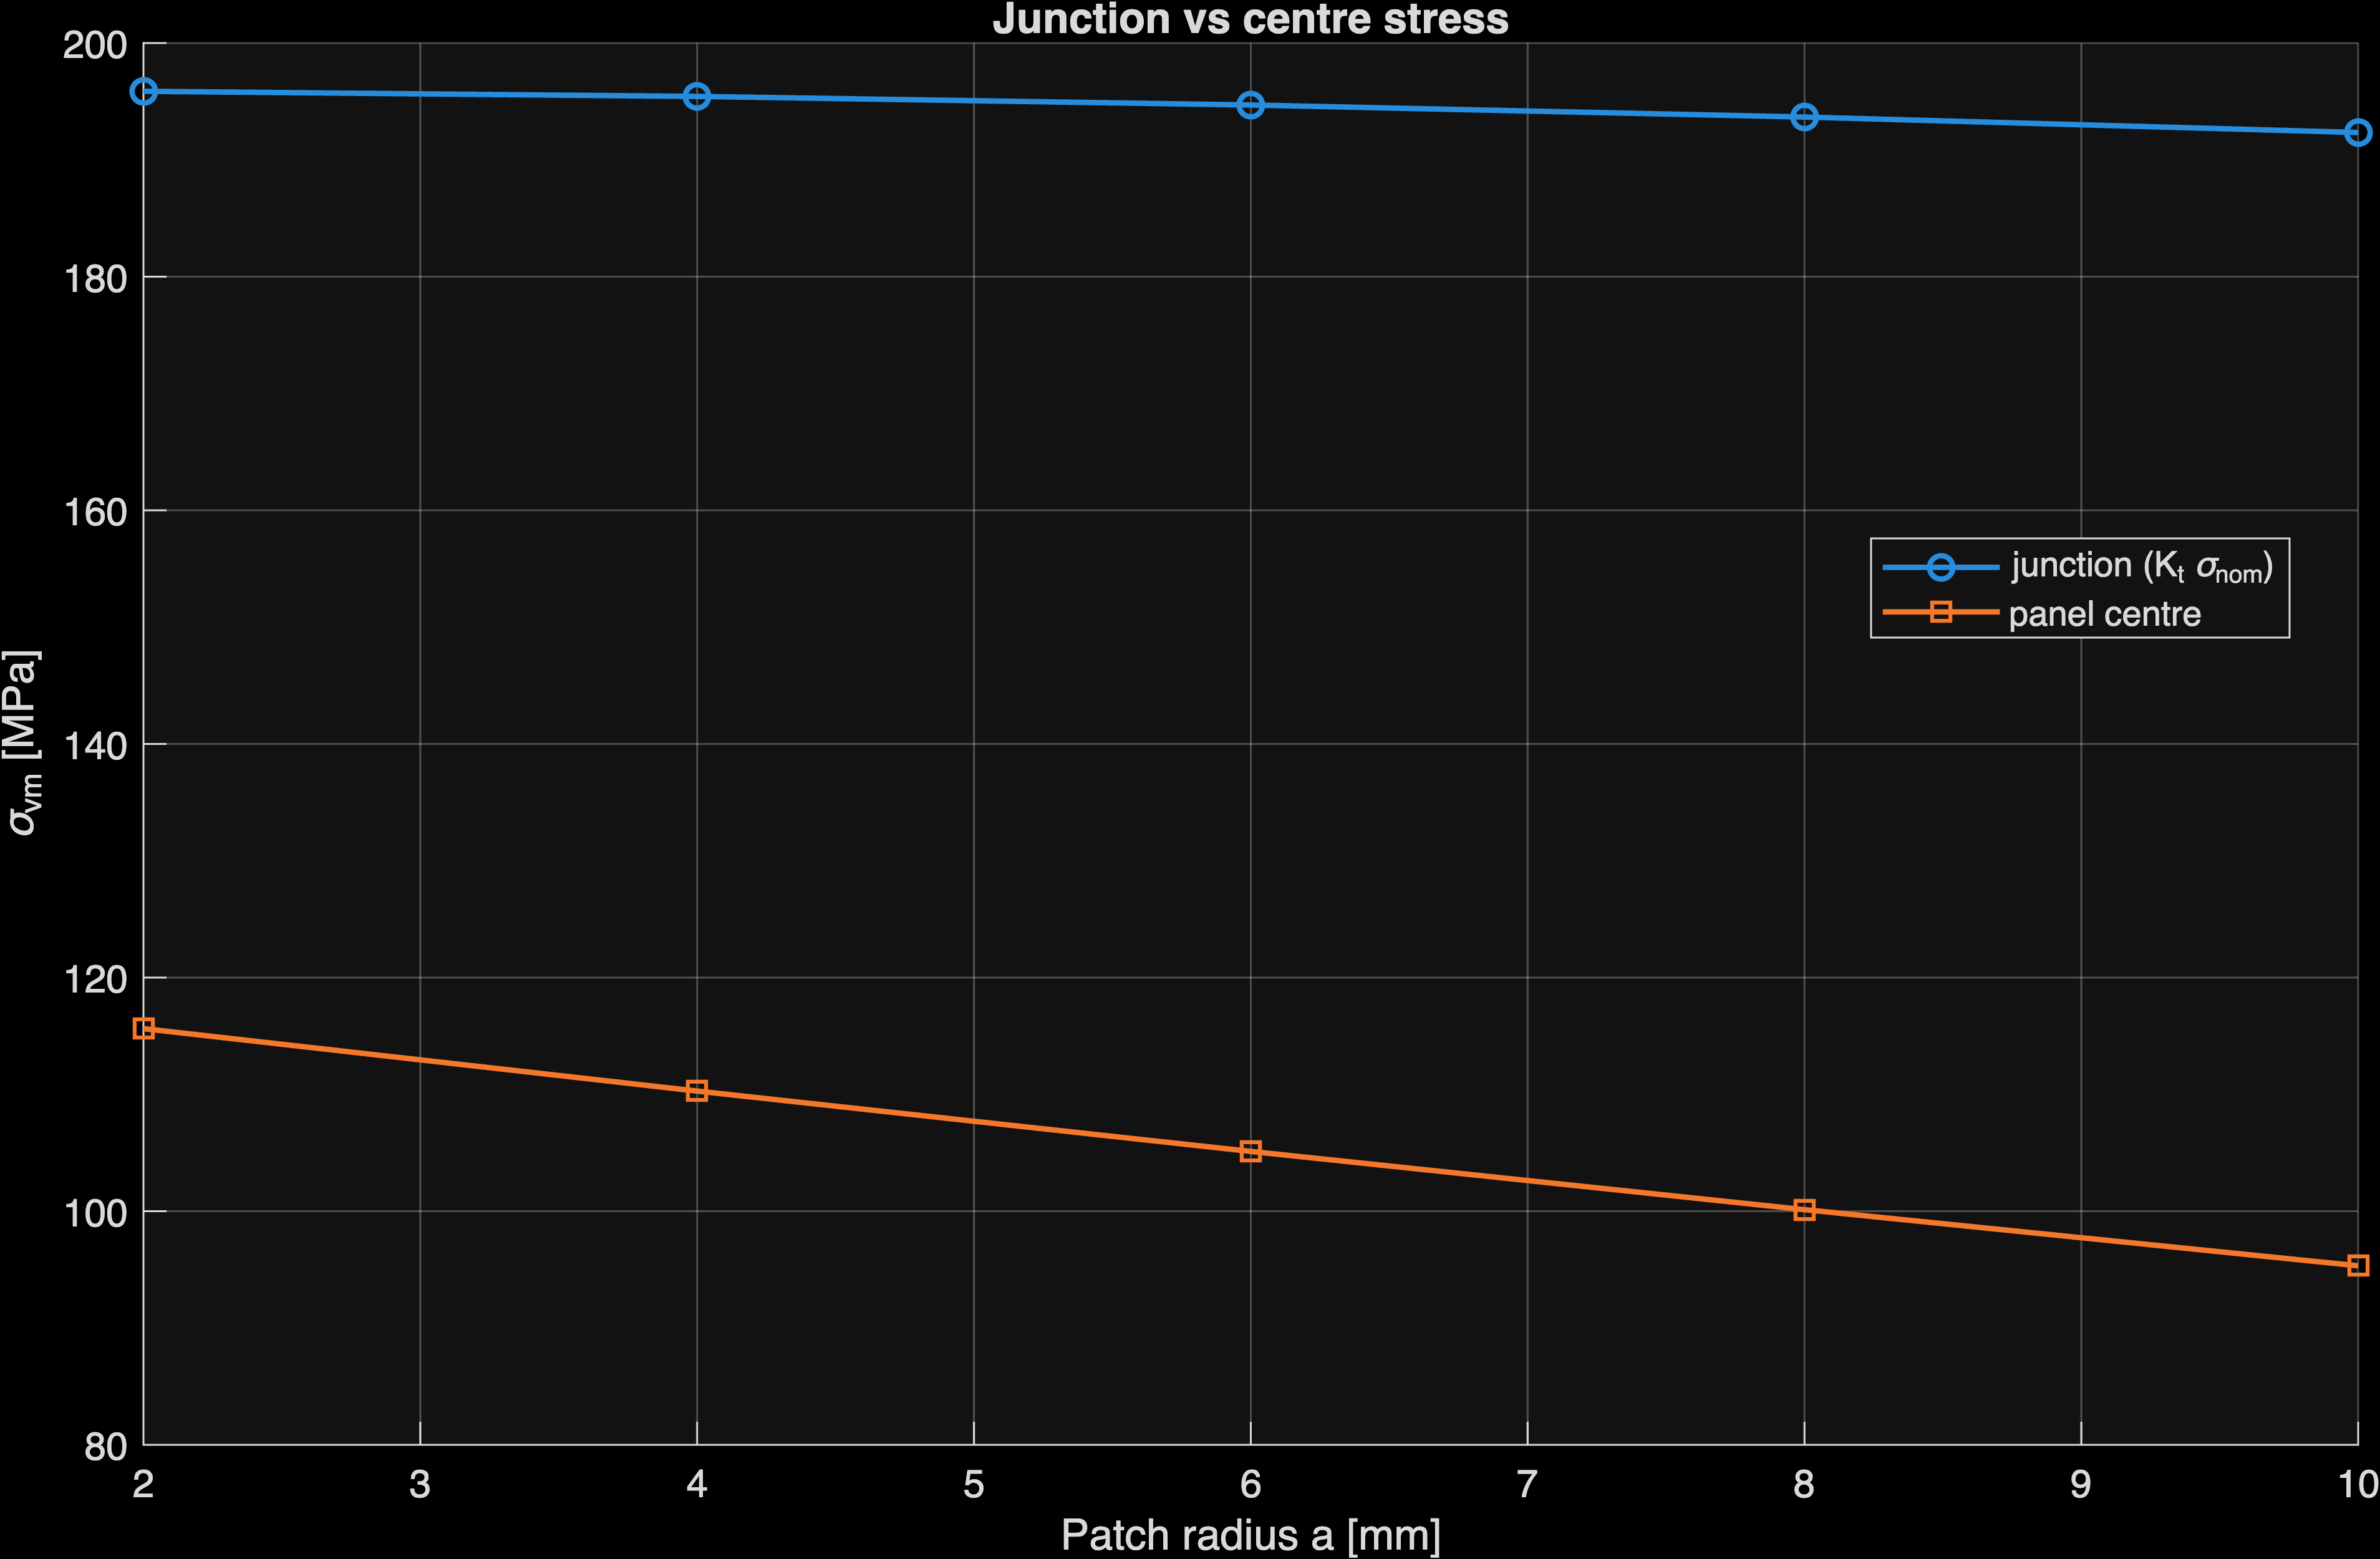
\includegraphics[width=\linewidth]{analytical_peak_stress_vs_a.png}
    \caption{Junction and centre peaks against $a$}
  \end{subfigure}
  \caption{Analytical results at \SI{400}{N}. Triangles mark $K_t\sigma$ at the junctions; the dotted line is the \SI{106}{MPa} fatigue limit.}
  \label{fig:analytical}
\end{figure}

\begin{table}[htbp]
  \centering
  \caption{Analytical summary at \SI{400}{N} (\href{\blob/scripts\%20and\%20outputs/tier_1/output/summary.csv}{\texttt{summary.csv}}). $\sigma_{\text{nom},j}$ is the bending stress $\sigma_x$ at the junction, before conversion to von Mises.}
  \label{tab:summary}
  \begin{tabular}{rrrrrr}
    \toprule
    $a$ (mm) & $M_j$ (N\,mm) & $\sigma_{\text{nom},j}$ (MPa) & $K_t\sigma_{\text{vm},j}$ (MPa) & $\sigma_{\text{vm},c}$ (MPa) & ratio $j/c$ \\
    \midrule
     2 & 3636 & 136.4 & 195.9 & 115.6 & 1.69 \\
     4 & 3628 & 136.1 & 195.4 & 110.3 & 1.77 \\
     6 & 3614 & 135.5 & 194.7 & 105.1 & 1.85 \\
     8 & 3595 & 134.8 & 193.7 & 100.1 & 1.93 \\
    10 & 3571 & 133.9 & 192.3 &  95.3 & 2.02 \\
    \bottomrule
  \end{tabular}
\end{table}

\subsection{FEA and mesh convergence}
Figure~\ref{fig:feapaths} shows the FEA stress along the path for all five patch radii on each mesh. Subscripts $j$ and $c$ are used throughout for the junction and the panel centre. The peaks were taken as the largest Total value within \SI{15}{mm} of either end (junction) and within $\pm\SI{10}{mm}$ of mid-span (centre).

On the \SI{10}{mm} mesh the curves are ragged and not ordered physically. The centre peak at $a = \SI{4}{mm}$ (\SI{36.7}{MPa}) is far below that at $a = \SI{6}{mm}$ (\SI{95.7}{MPa}), although spreading the same load over a larger patch can only lower the peak. On the \SI{1}{mm} and \SI{0.1}{mm} meshes the curves are smooth and correctly ordered ($\sigma_{\text{vm},c}$ falls monotonically with $a$), and the two meshes are almost indistinguishable at the centre. The junction peak appears as a sharp spike at $S \approx \SI{7}{mm}$ (and symmetrically near the far end), and it is nearly independent of $a$, as the beam model predicts.

\begin{figure}[htbp]
  \centering
  \begin{subfigure}[b]{0.45\textwidth}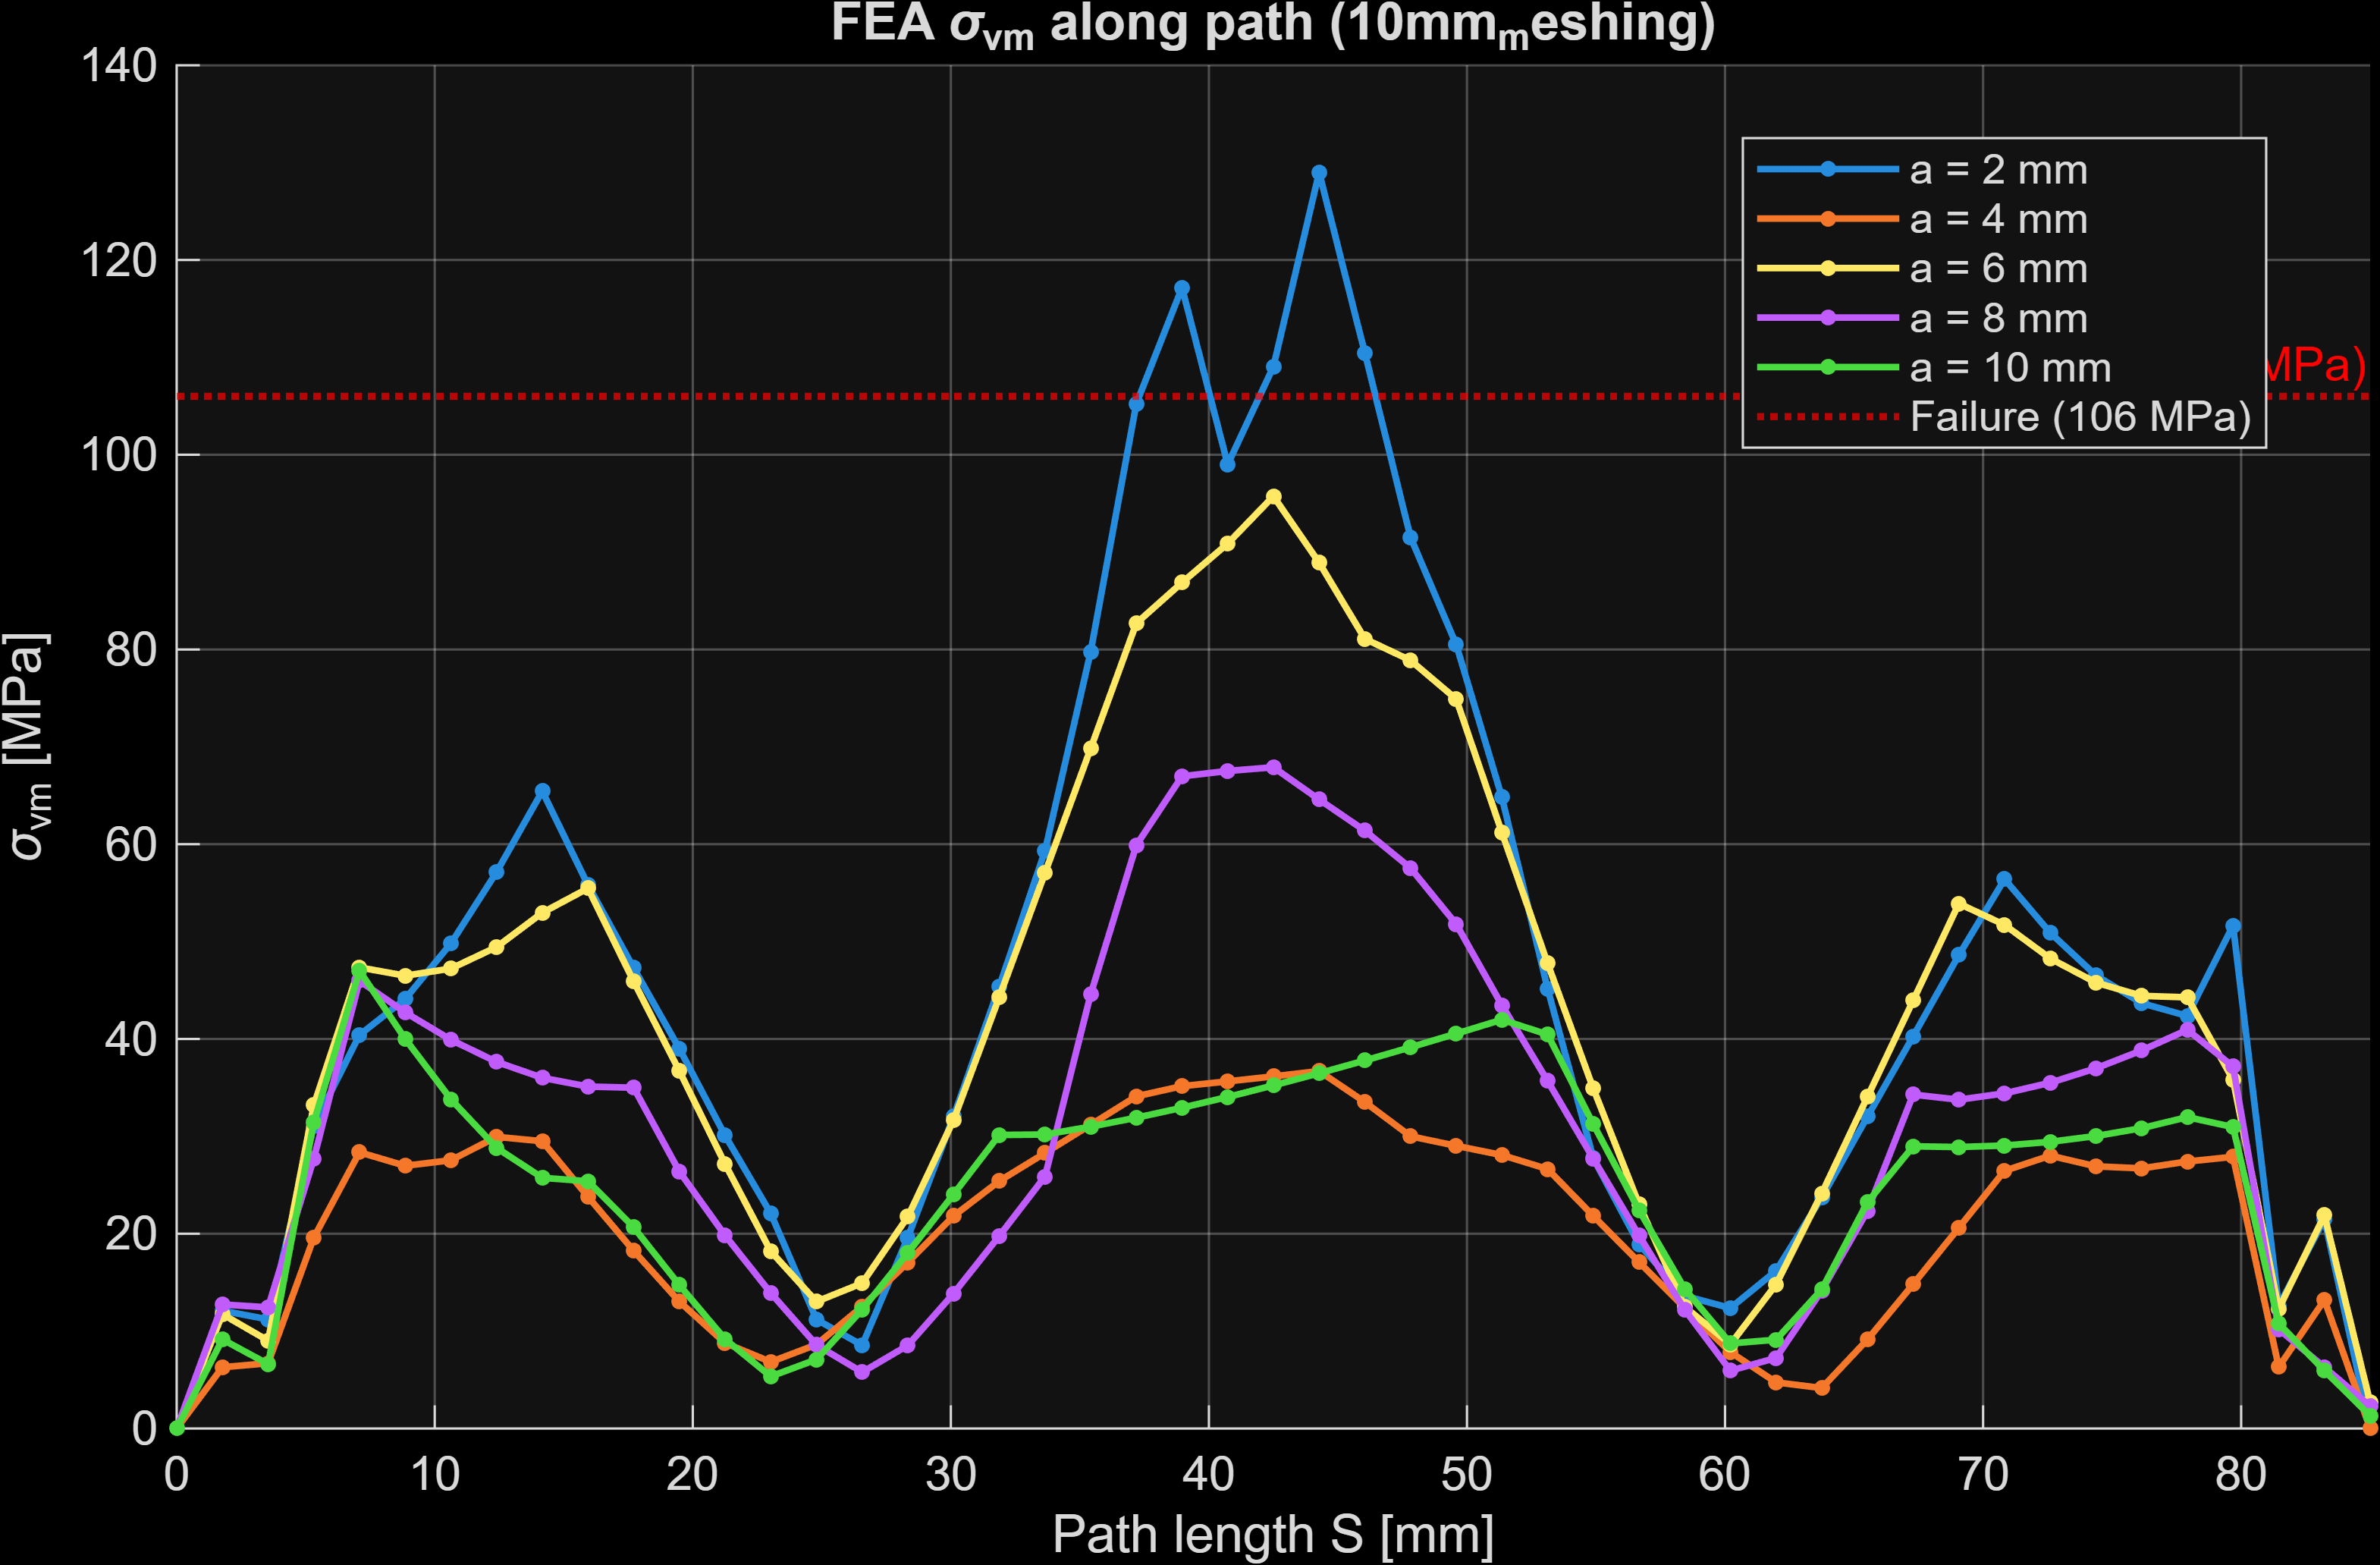
\includegraphics[width=\linewidth]{10mm_meshing/fea_path_stress_vs_x.png}\caption{\SI{10}{mm} mesh}\end{subfigure}\hfill
  \begin{subfigure}[b]{0.45\textwidth}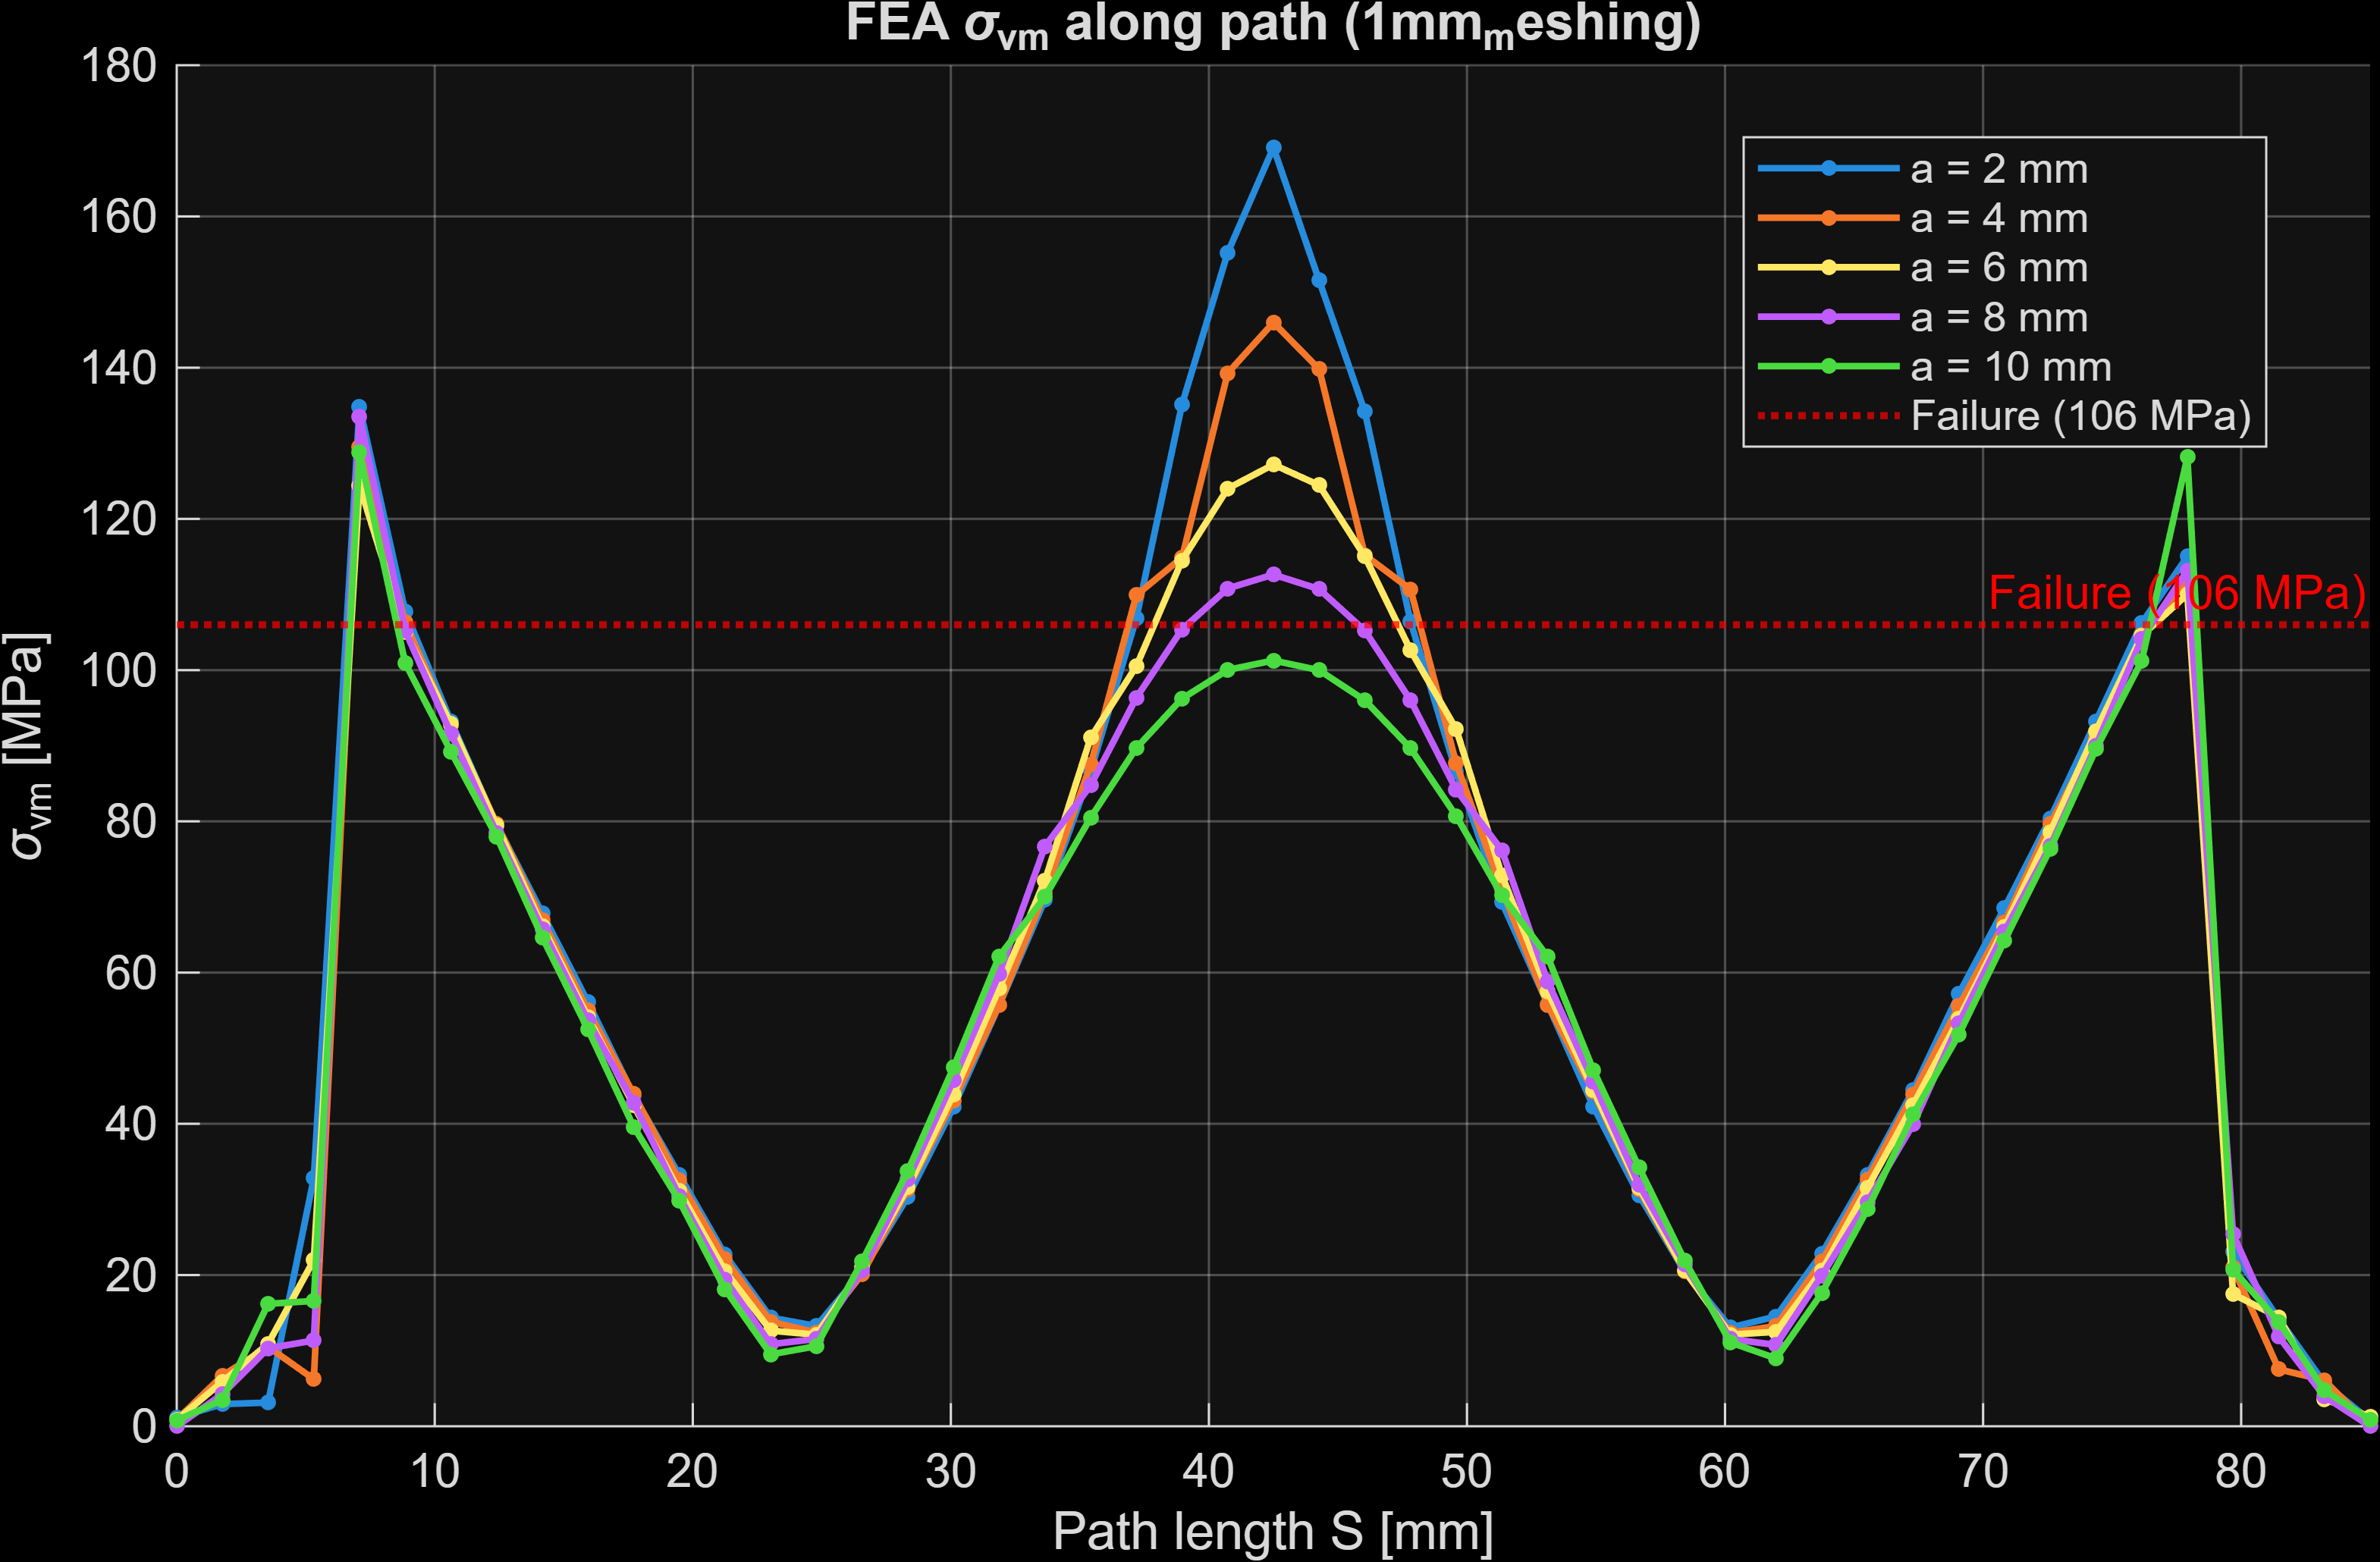
\includegraphics[width=\linewidth]{1mm_meshing/fea_path_stress_vs_x.png}\caption{\SI{1}{mm} mesh}\end{subfigure}\\[4pt]
  \begin{subfigure}[b]{0.45\textwidth}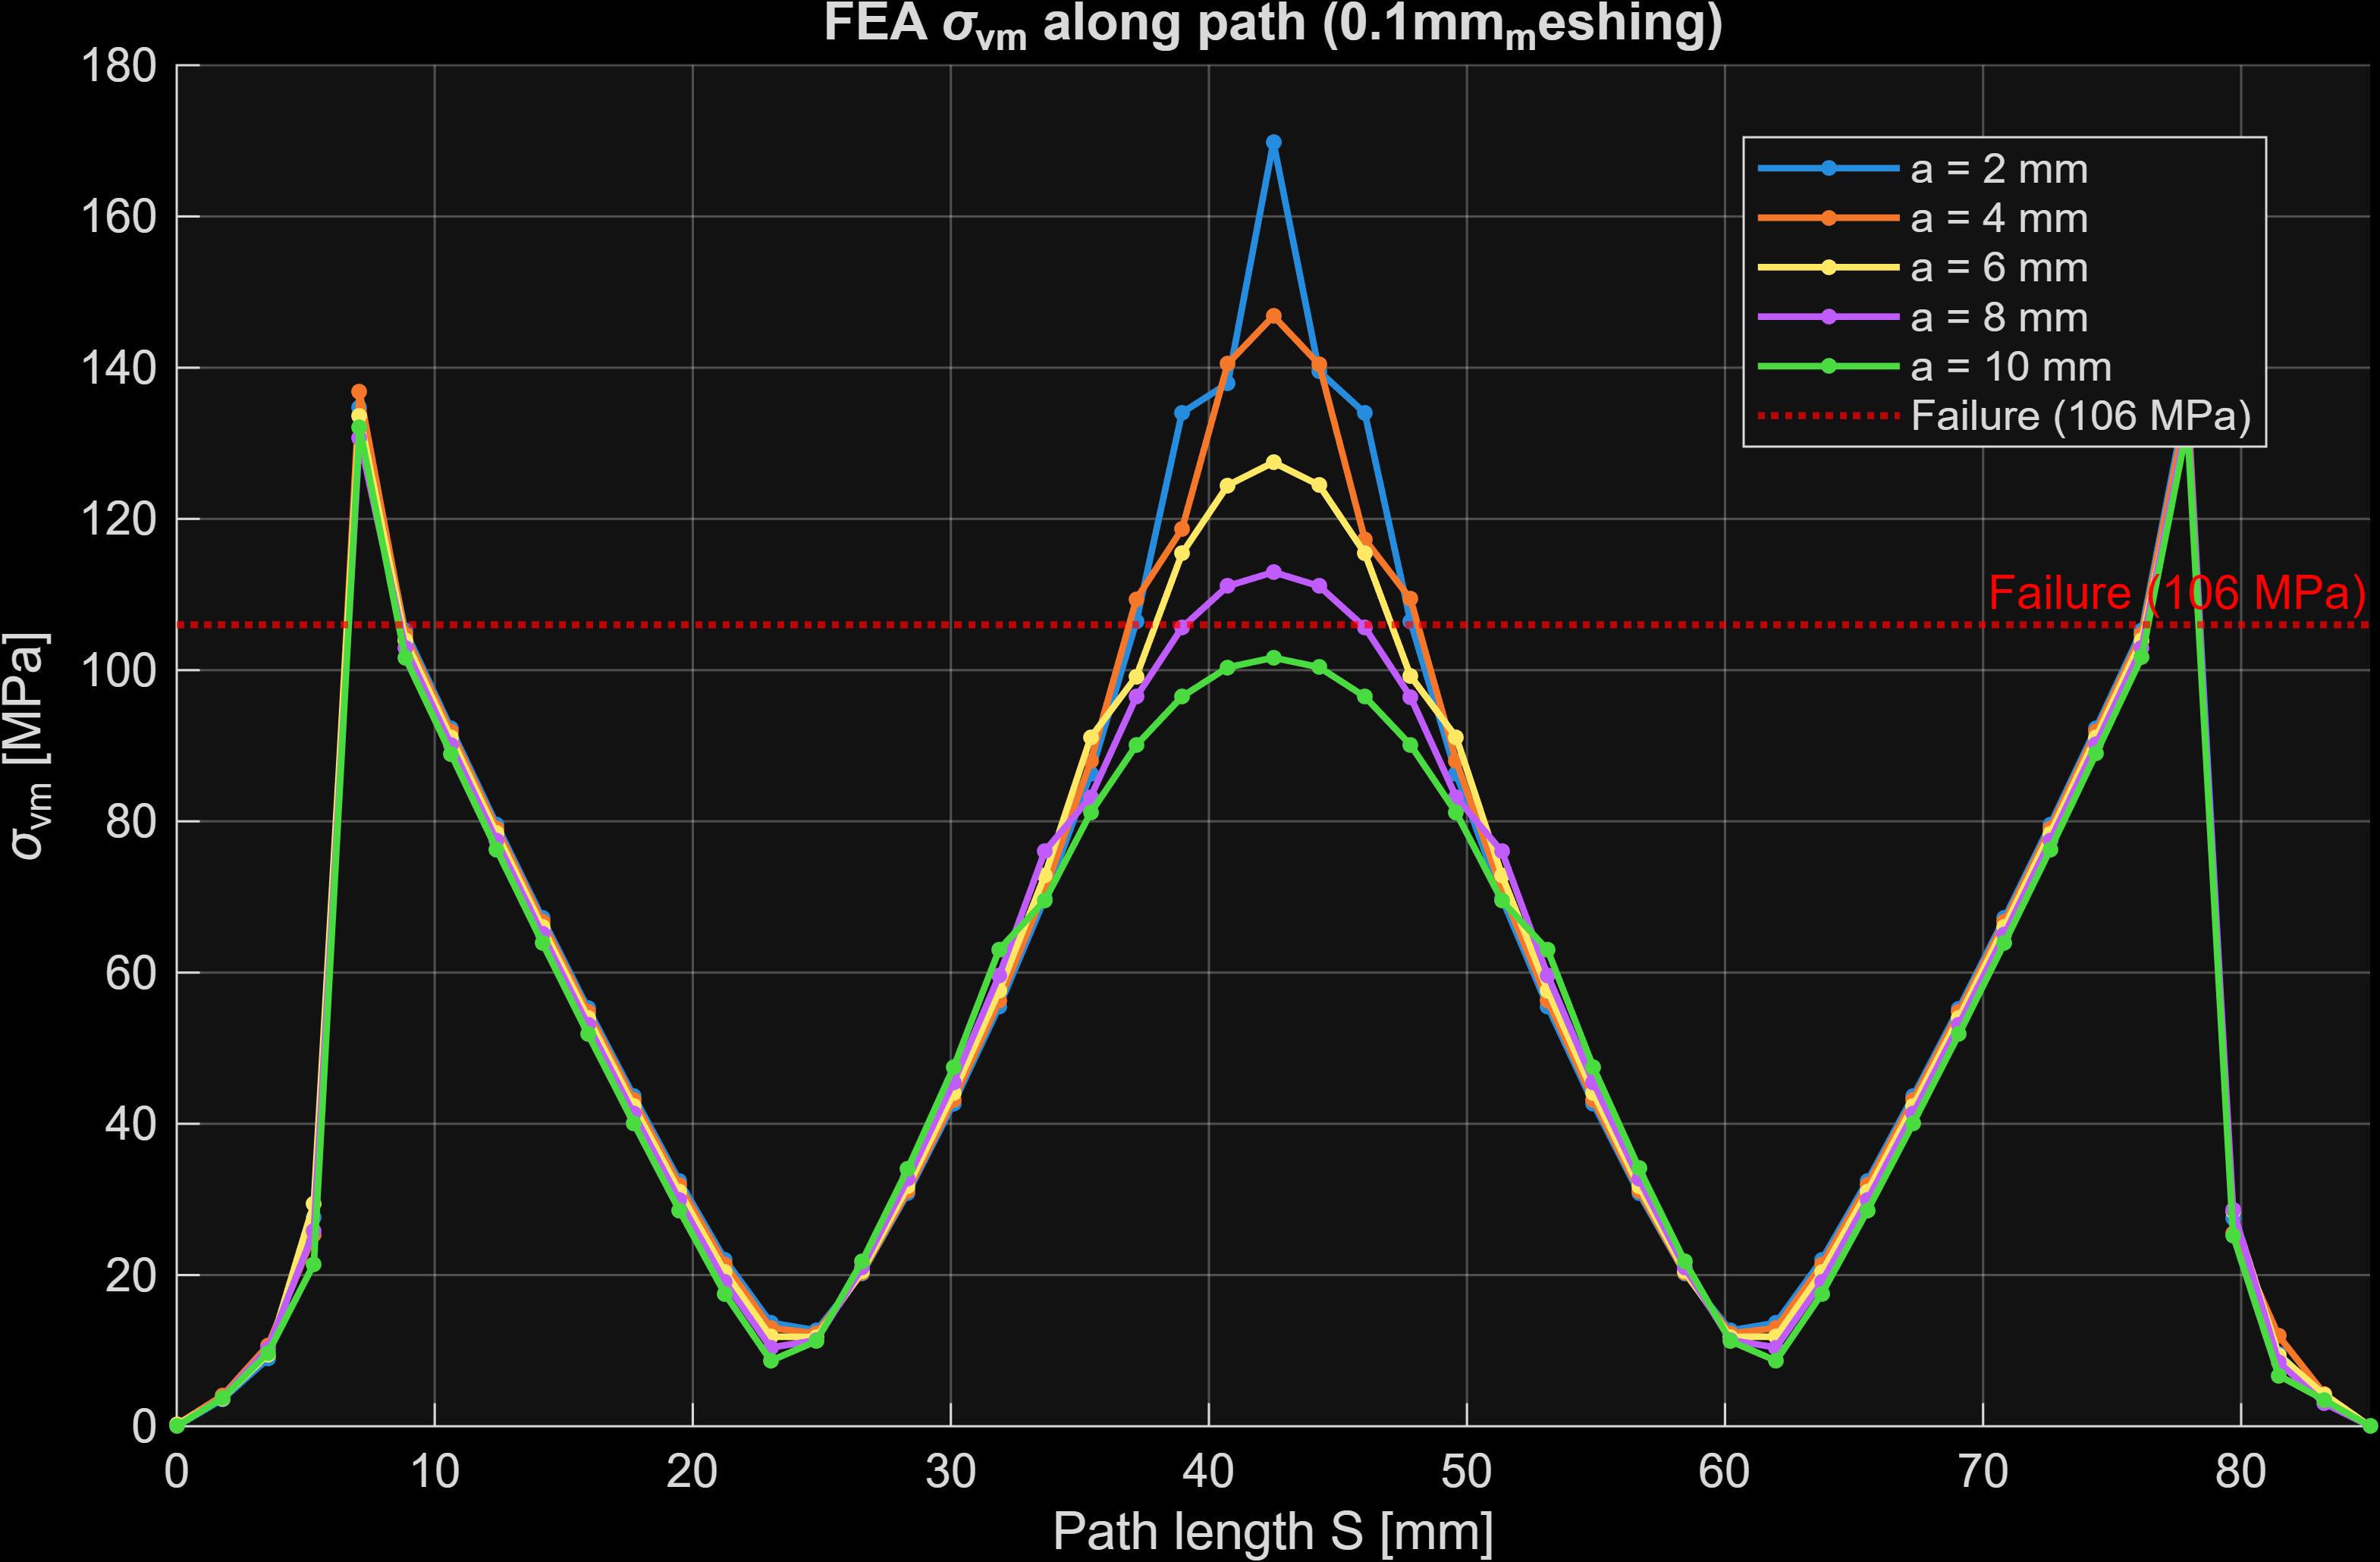
\includegraphics[width=\linewidth]{0.1mm_meshing/fea_path_stress_vs_x.png}\caption{\SI{0.1}{mm} mesh}\end{subfigure}
  \caption{FEA Total $\sigma_\text{vm}$ along the path for $a = 2$--\SI{10}{mm}, scaled to \SI{400}{N}, on each mesh.}
  \label{fig:feapaths}
\end{figure}

Table~\ref{tab:conv} quantifies the convergence. Going from \SI{10}{mm} to \SI{1}{mm}, the centre peak rises by \SI{31}{\percent} to \SI{298}{\percent} and the junction peak by \SI{106}{\percent} to \SI{332}{\percent}: the coarse mesh cannot represent bending of a \SI{2}{mm} skin, and for the smaller patches the loaded area is smaller than one element, so the stresses it returns are far too low. Going on from \SI{1}{mm} to \SI{0.1}{mm}, the centre peak changes by only \SI{0.2}{\percent}--\SI{0.6}{\percent}, which is converged for engineering purposes. The junction peak changes by up to \SI{7.4}{\percent} and always upward (except $a = \SI{8}{mm}$, $-\SI{0.2}{\percent}$): it converges more slowly because a \SI{1}{mm} element is as large as the \SI{1}{mm} fillet that creates the concentration.

The apparent order of convergence, $p = \ln\!\big[(f_{1}-f_{10})/(f_{0.1}-f_{1})\big]/\ln 10$ with $f_h$ the peak on the mesh of size $h$, is about 2 for the centre (1.8--2.2) and between 0.9 and 1.7 for the junction ($a = \SI{8}{mm}$ is not monotonic, so $p$ is undefined). Since the coarsest mesh is far outside the asymptotic range, $p$ is only indicative. If the trend continues, the residual error of the \SI{0.1}{mm} mesh, $(f_{0.1}-f_{1})/(10^p-1)$, is below \SI{0.1}{MPa} at the centre and about \SI{1.4}{MPa} (\SI{1}{\percent}) or less at the junction. Figure~\ref{fig:conv} shows the same behaviour graphically: every curve is steep between \SI{10}{mm} and \SI{1}{mm} and flat between \SI{1}{mm} and \SI{0.1}{mm}, with the junction curves not quite flat. Figure~\ref{fig:overlaya2} shows what this means for one case: for $a = \SI{2}{mm}$ the FEA curve climbs towards its converged shape as the mesh is refined, and almost stops changing between the last two meshes.

\begin{table}[htbp]
  \centering
  \caption{FEA peak $\sigma_\text{vm}$ (MPa, at \SI{400}{N}) on each mesh, the change on the last refinement step, and the apparent order of convergence $p$ (\href{\blob/scripts\%20and\%20outputs/tier_1/output}{\texttt{fea\_vs\_analytical.csv}} in each mesh folder). Changes are in percent.}
  \label{tab:conv}
  \begin{tabular}{rrrrrrr}
    \toprule
    $a$ (mm) & \SI{10}{mm} & \SI{1}{mm} & \SI{0.1}{mm} & $\Delta_{10\to1}$ (\%) & $\Delta_{1\to0.1}$ (\%) & $p$ \\
    \midrule
    \multicolumn{7}{l}{\emph{Panel centre}} \\
    2 & 129.0 & 169.1 & 169.8 & +31 & +0.41 & 1.76 \\
    4 & 36.7 & 146.0 & 146.8 & +298 & +0.59 & 2.10 \\
    6 & 95.7 & 127.2 & 127.5 & +33 & +0.23 & 2.04 \\
    8 & 67.9 & 112.6 & 113.0 & +66 & +0.28 & 2.15 \\
    10 & 42.0 & 101.3 & 101.6 & +141 & +0.37 & 2.20 \\
    \midrule
    \multicolumn{7}{l}{\emph{Junction}} \\
    2 & 65.4 & 134.9 & 136.3 & +106 & +1.05 & 1.69 \\
    4 & 29.9 & 129.5 & 136.9 & +332 & +5.67 & 1.13 \\
    6 & 53.0 & 124.4 & 133.6 & +135 & +7.38 & 0.89 \\
    8 & 46.0 & 133.6 & 133.2 & +191 & $-$0.24 & -- \\
    10 & 47.0 & 128.8 & 132.3 & +174 & +2.70 & 1.37 \\
    \bottomrule
  \end{tabular}
\end{table}

\begin{figure}[htbp]
  \centering
  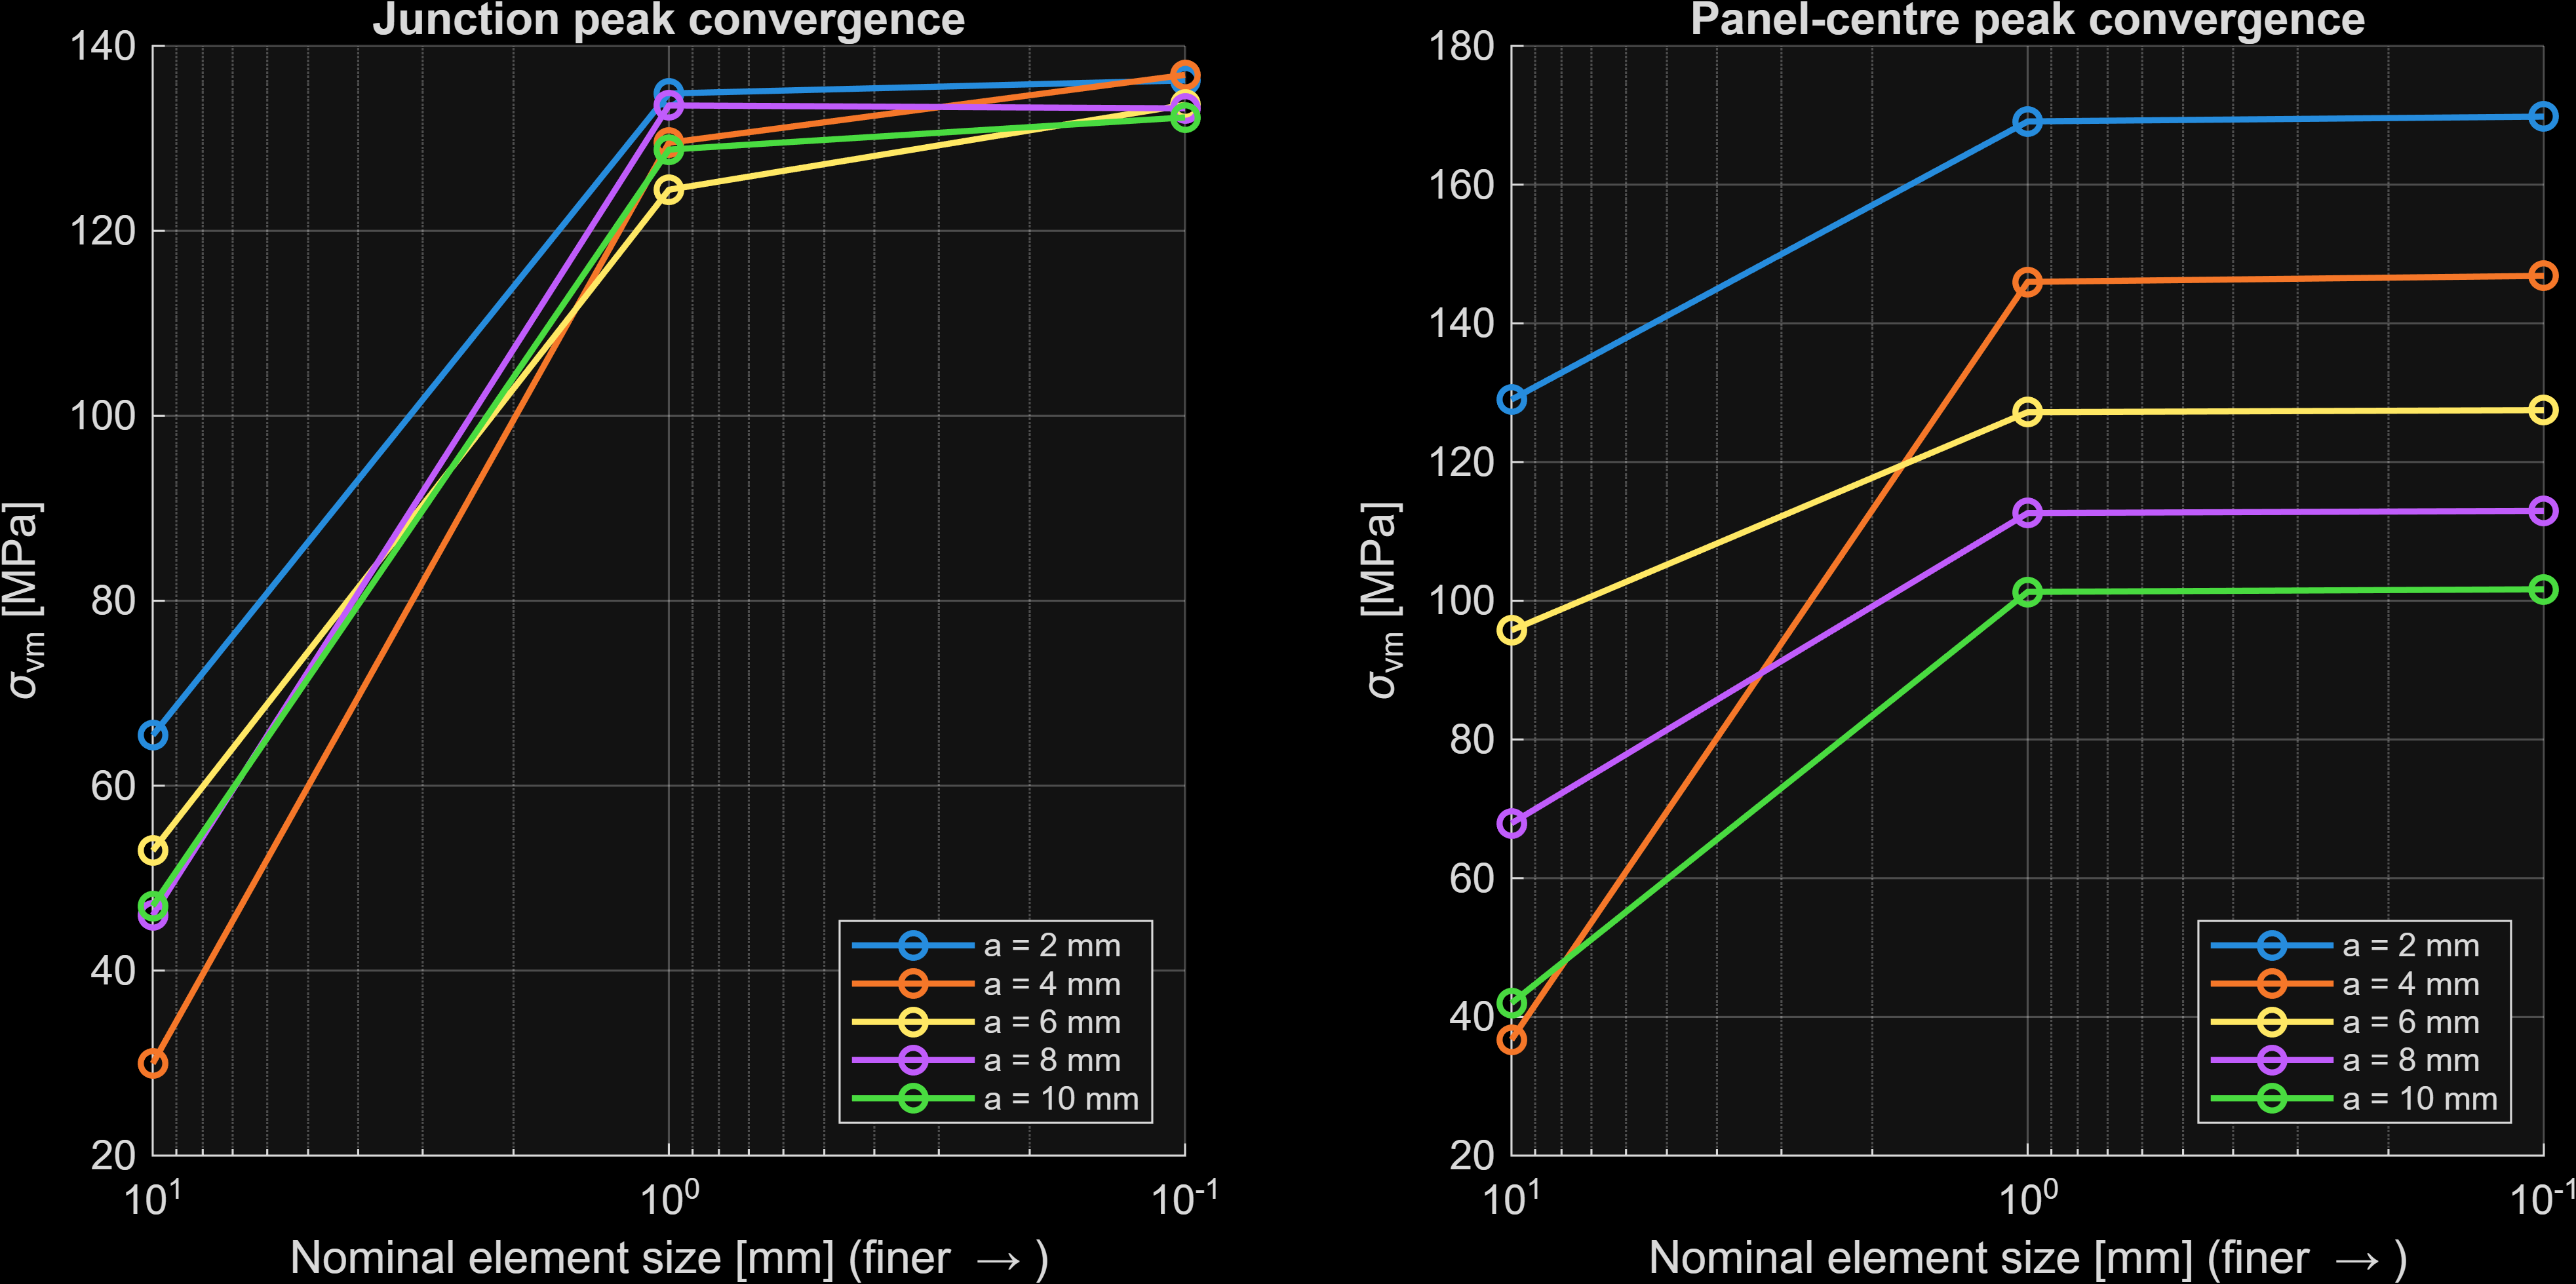
\includegraphics[width=0.8\textwidth]{mesh_convergence.png}
  \caption{Mesh convergence of the FEA peaks: junction (left) and panel centre (right) against nominal element size, one curve per patch radius, at \SI{400}{N}.}
  \label{fig:conv}
\end{figure}

\begin{figure}[t]
  \centering
  \begin{subfigure}[b]{0.32\textwidth}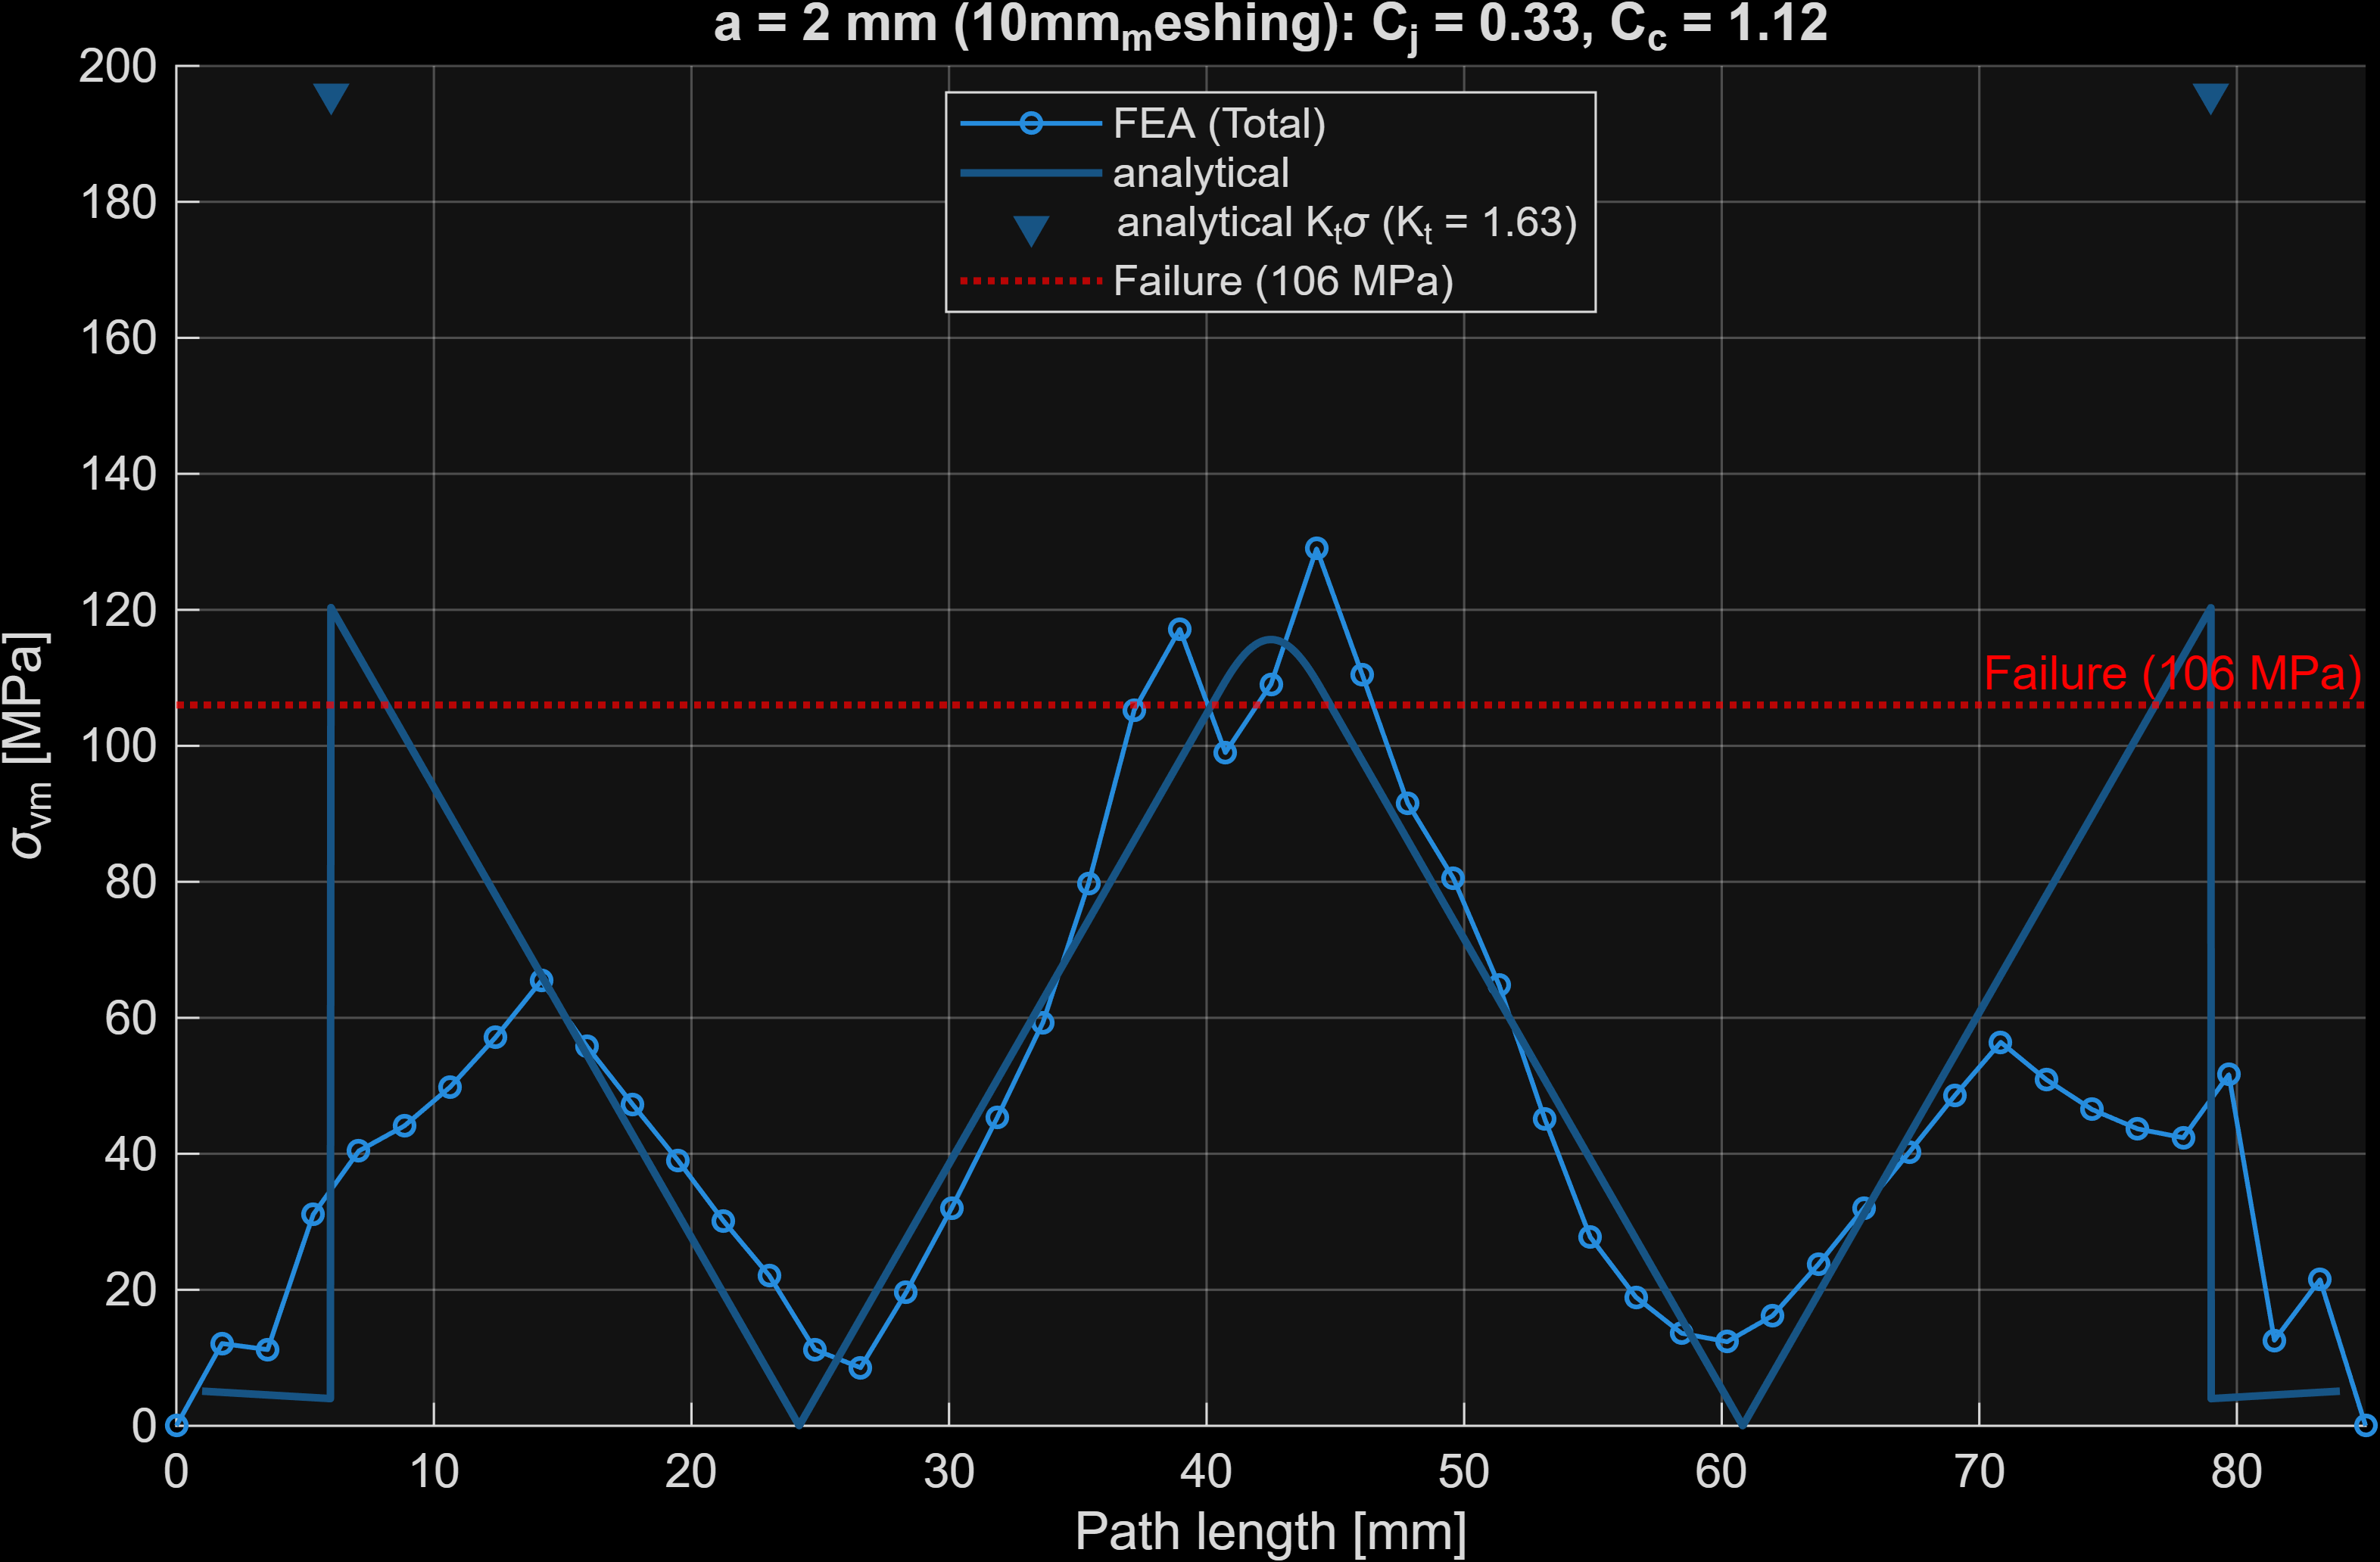
\includegraphics[width=\linewidth]{10mm_meshing/overlay_a2.png}\caption{\SI{10}{mm} mesh}\end{subfigure}\hfill
  \begin{subfigure}[b]{0.32\textwidth}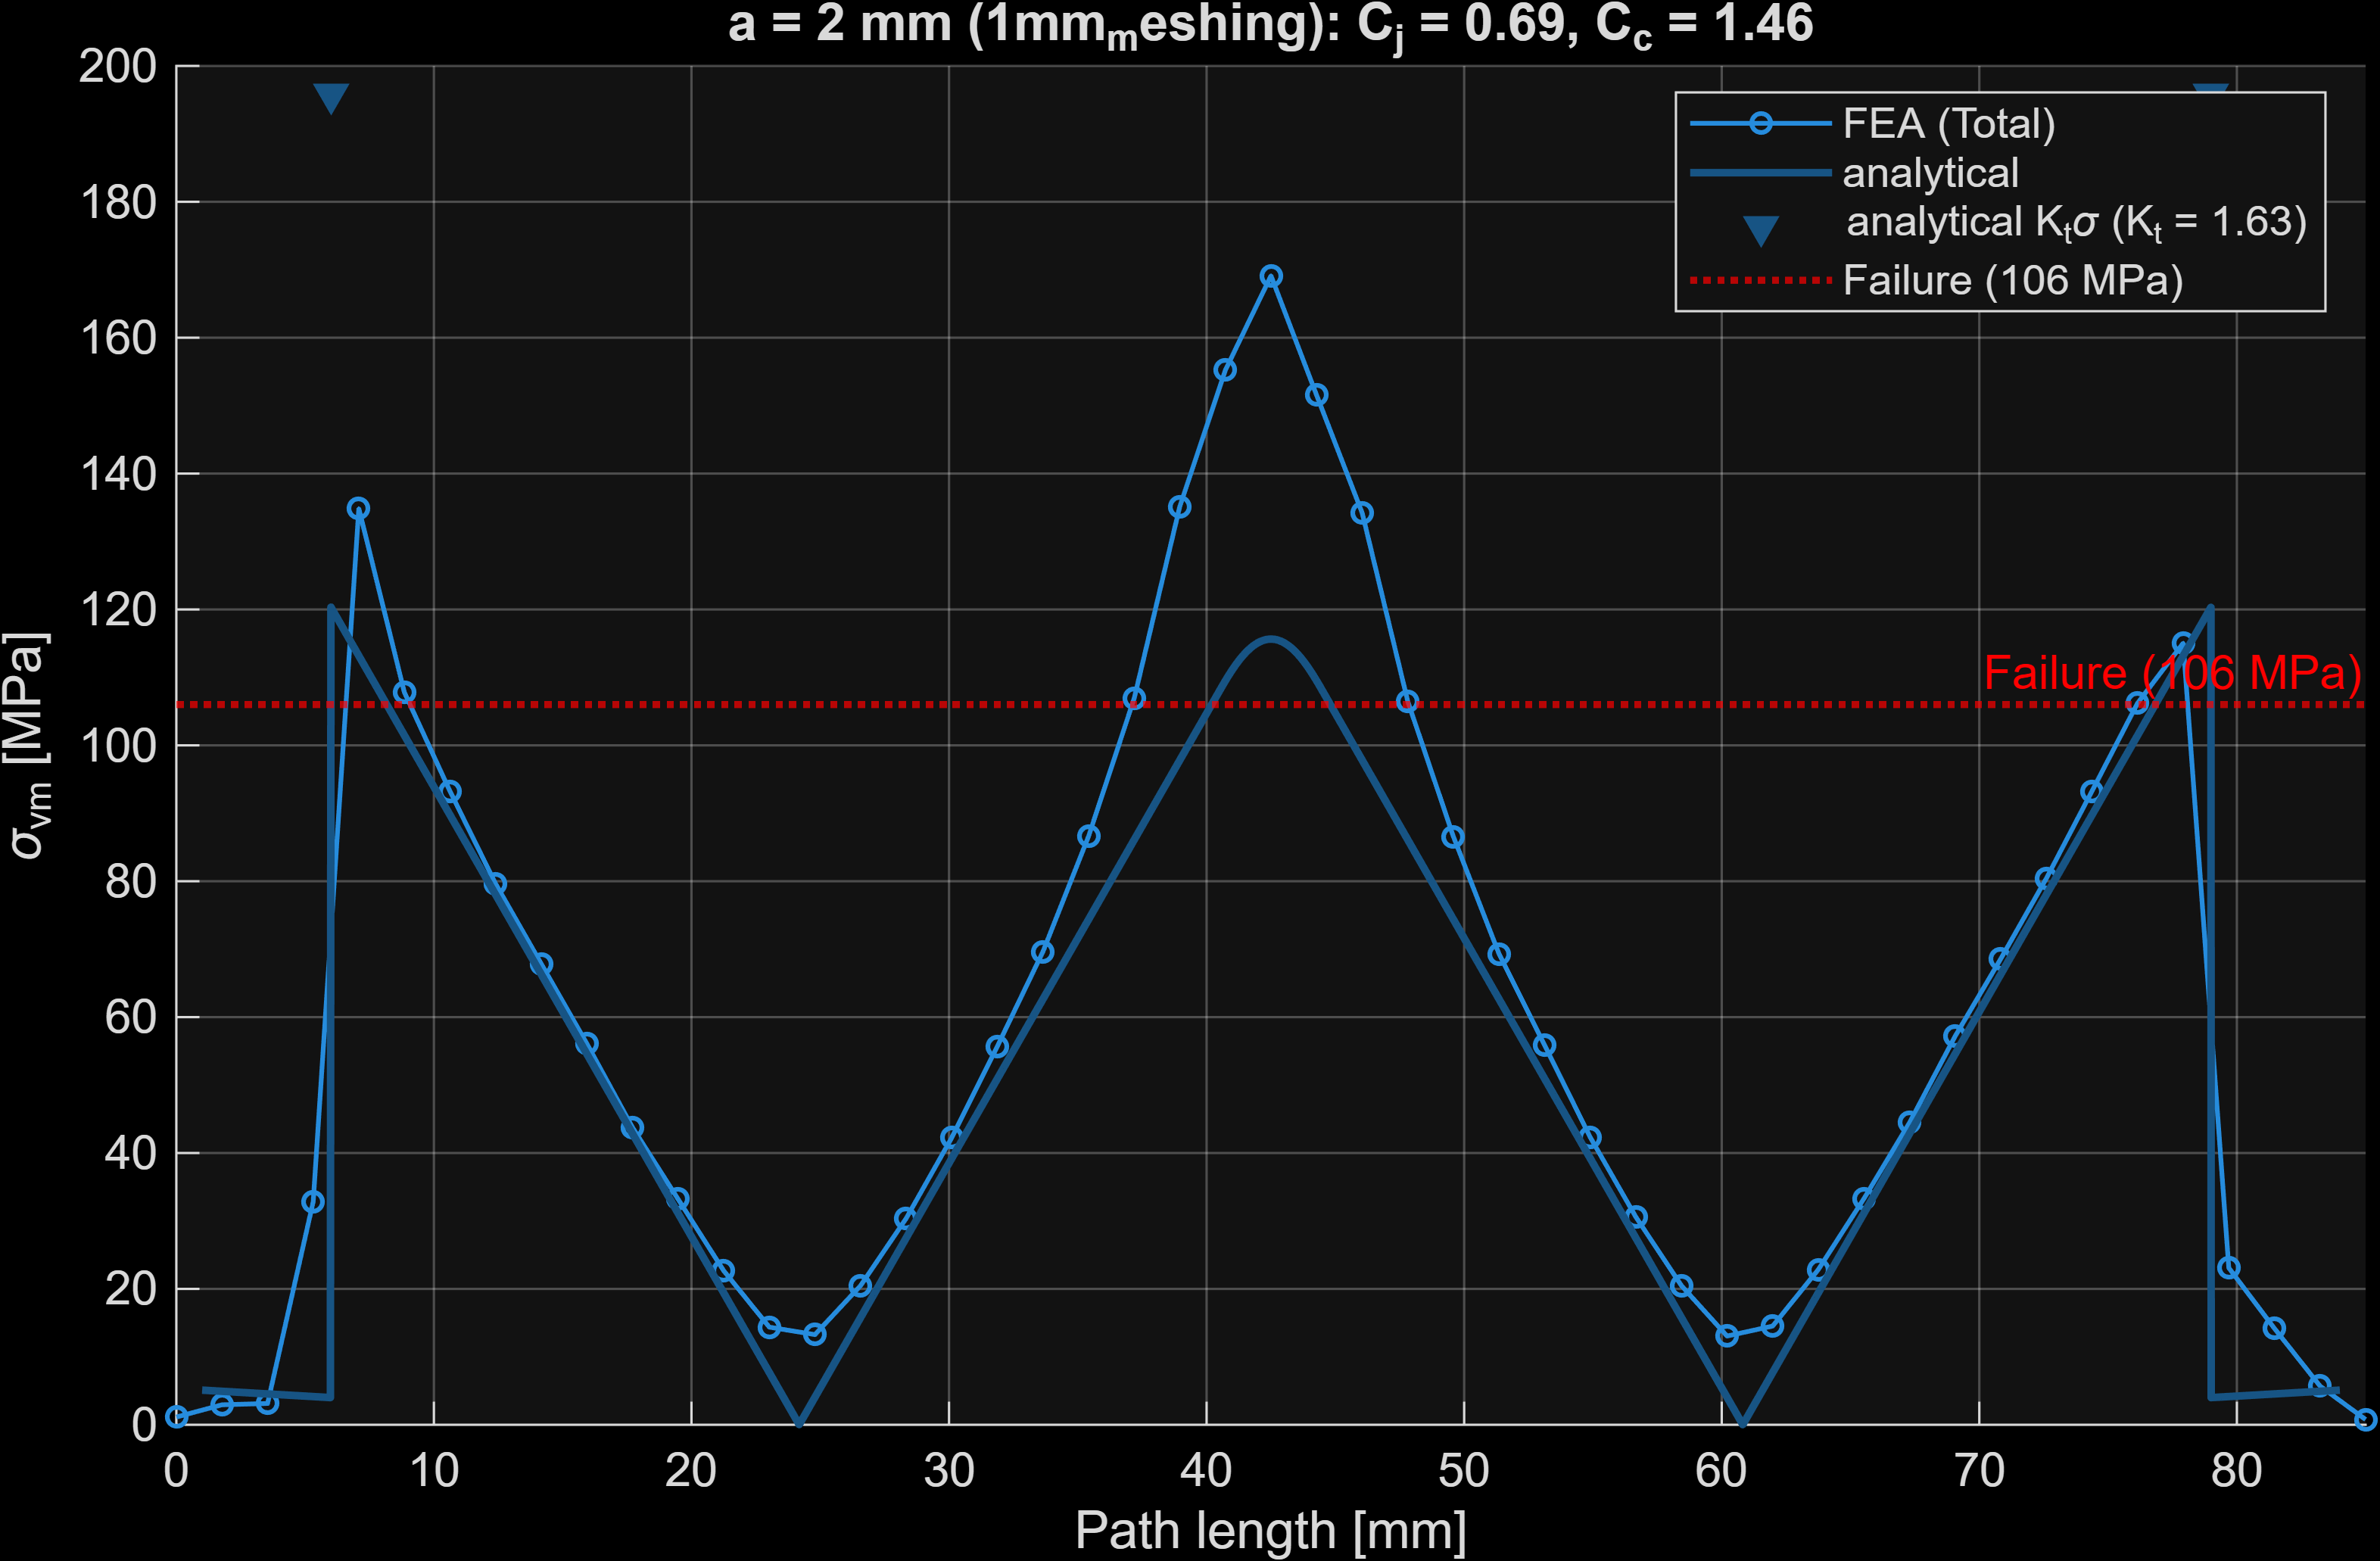
\includegraphics[width=\linewidth]{1mm_meshing/overlay_a2.png}\caption{\SI{1}{mm} mesh}\end{subfigure}\hfill
  \begin{subfigure}[b]{0.32\textwidth}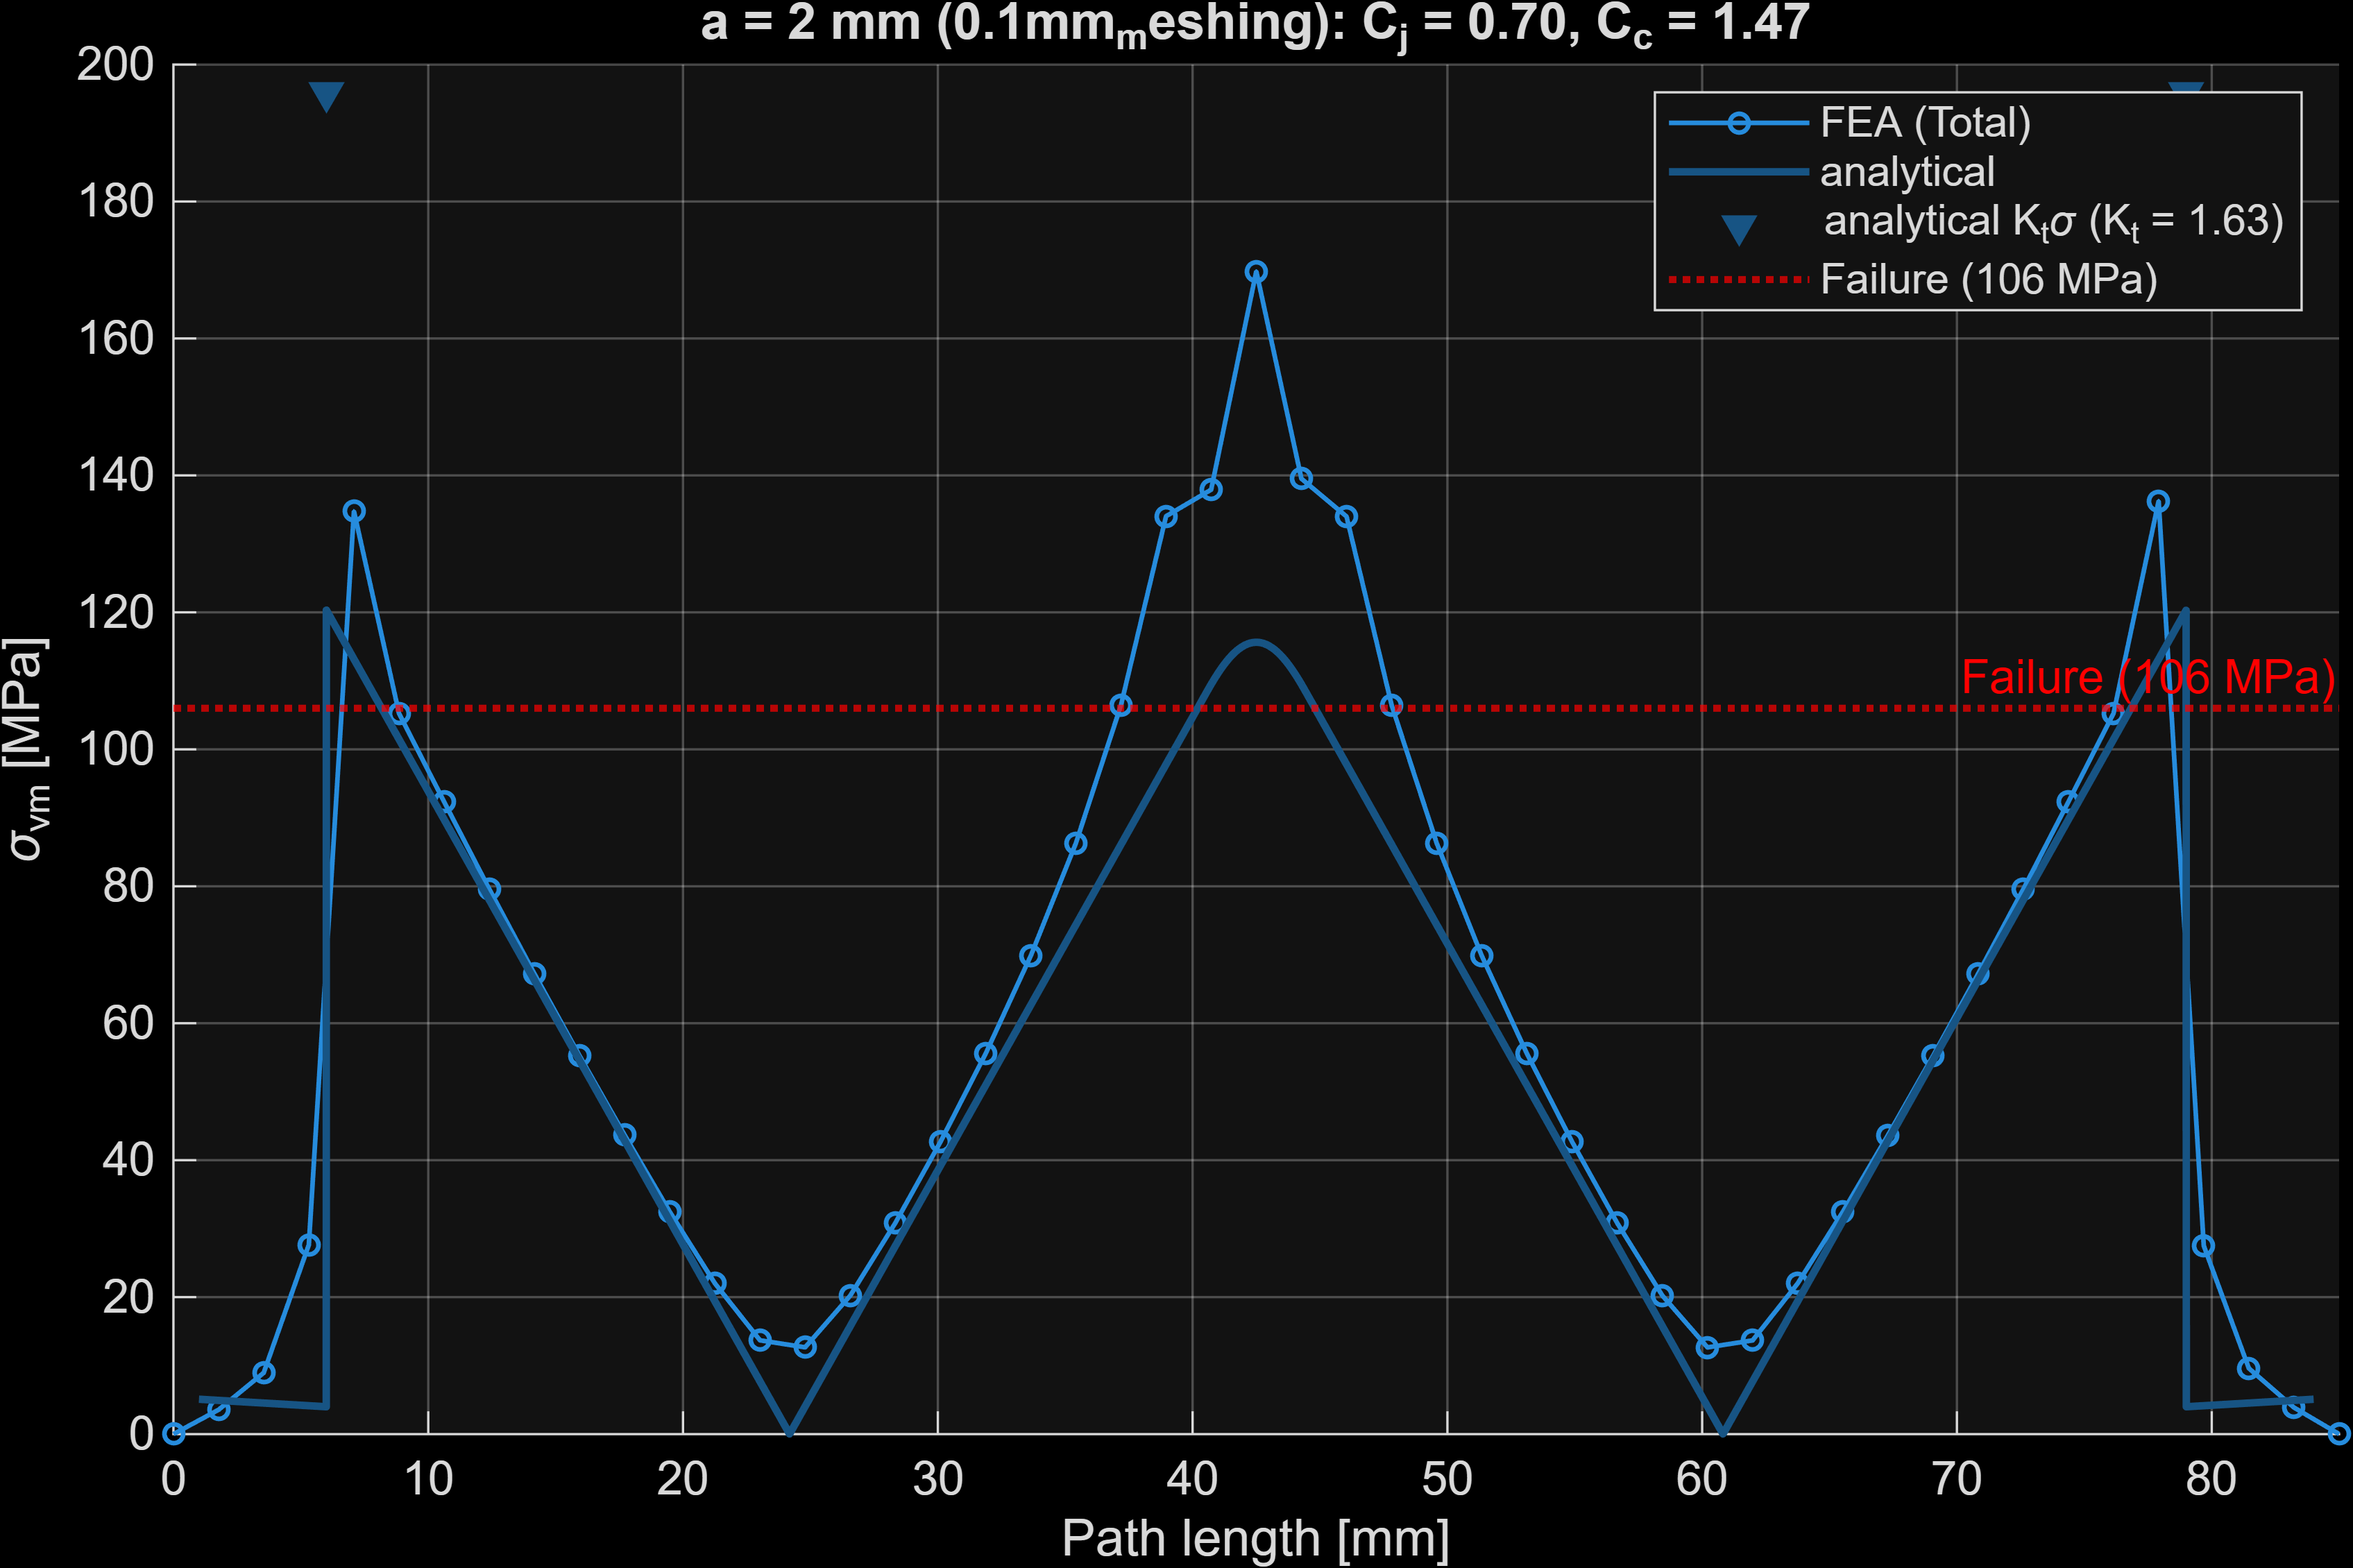
\includegraphics[width=\linewidth]{0.1mm_meshing/overlay_a2.png}\caption{\SI{0.1}{mm} mesh}\end{subfigure}
  \caption{FEA against analytical $\sigma_\text{vm}$ for $a = \SI{2}{mm}$ on each mesh: as the mesh is refined the FEA curve moves up to its converged shape.}
  \label{fig:overlaya2}
\end{figure}

Figure~\ref{fig:overlaya2} makes the same point against the analytical curve for the sharpest patch, $a = \SI{2}{mm}$: on the \SI{10}{mm} mesh the FEA curve is far below the beam solution and misses the centre peak, on the \SI{1}{mm} mesh it has already reached its final shape, and on the \SI{0.1}{mm} mesh it differs from that only in the junction peak.



\subsection{Comparison and calibration}
Figure~\ref{fig:peaks} overlays the FEA peaks from the three meshes on the analytical values, and Table~\ref{tab:calibmesh} gives the calibration factor $C = \sigma_\text{FEA}/\sigma_\text{analytical}$ for each mesh. The \SI{1}{mm} and \SI{0.1}{mm} meshes give practically the same $C_c$, and $C_j$ within about \SI{7}{\percent}, while the \SI{10}{mm} mesh gives values that are too low by \SI{25}{\percent} to \SI{75}{\percent} at the centre and by a factor of two to almost five at the junction, and are not monotonic in $a$. Table~\ref{tab:calib} gives the full comparison on the converged \SI{0.1}{mm} mesh, and Figure~\ref{fig:overlays} overlays the two solutions for each radius. The analytical span (\SI{83}{mm}) is centred on the \SI{85}{mm} FEA path.

\begin{figure}[htbp]
  \centering
  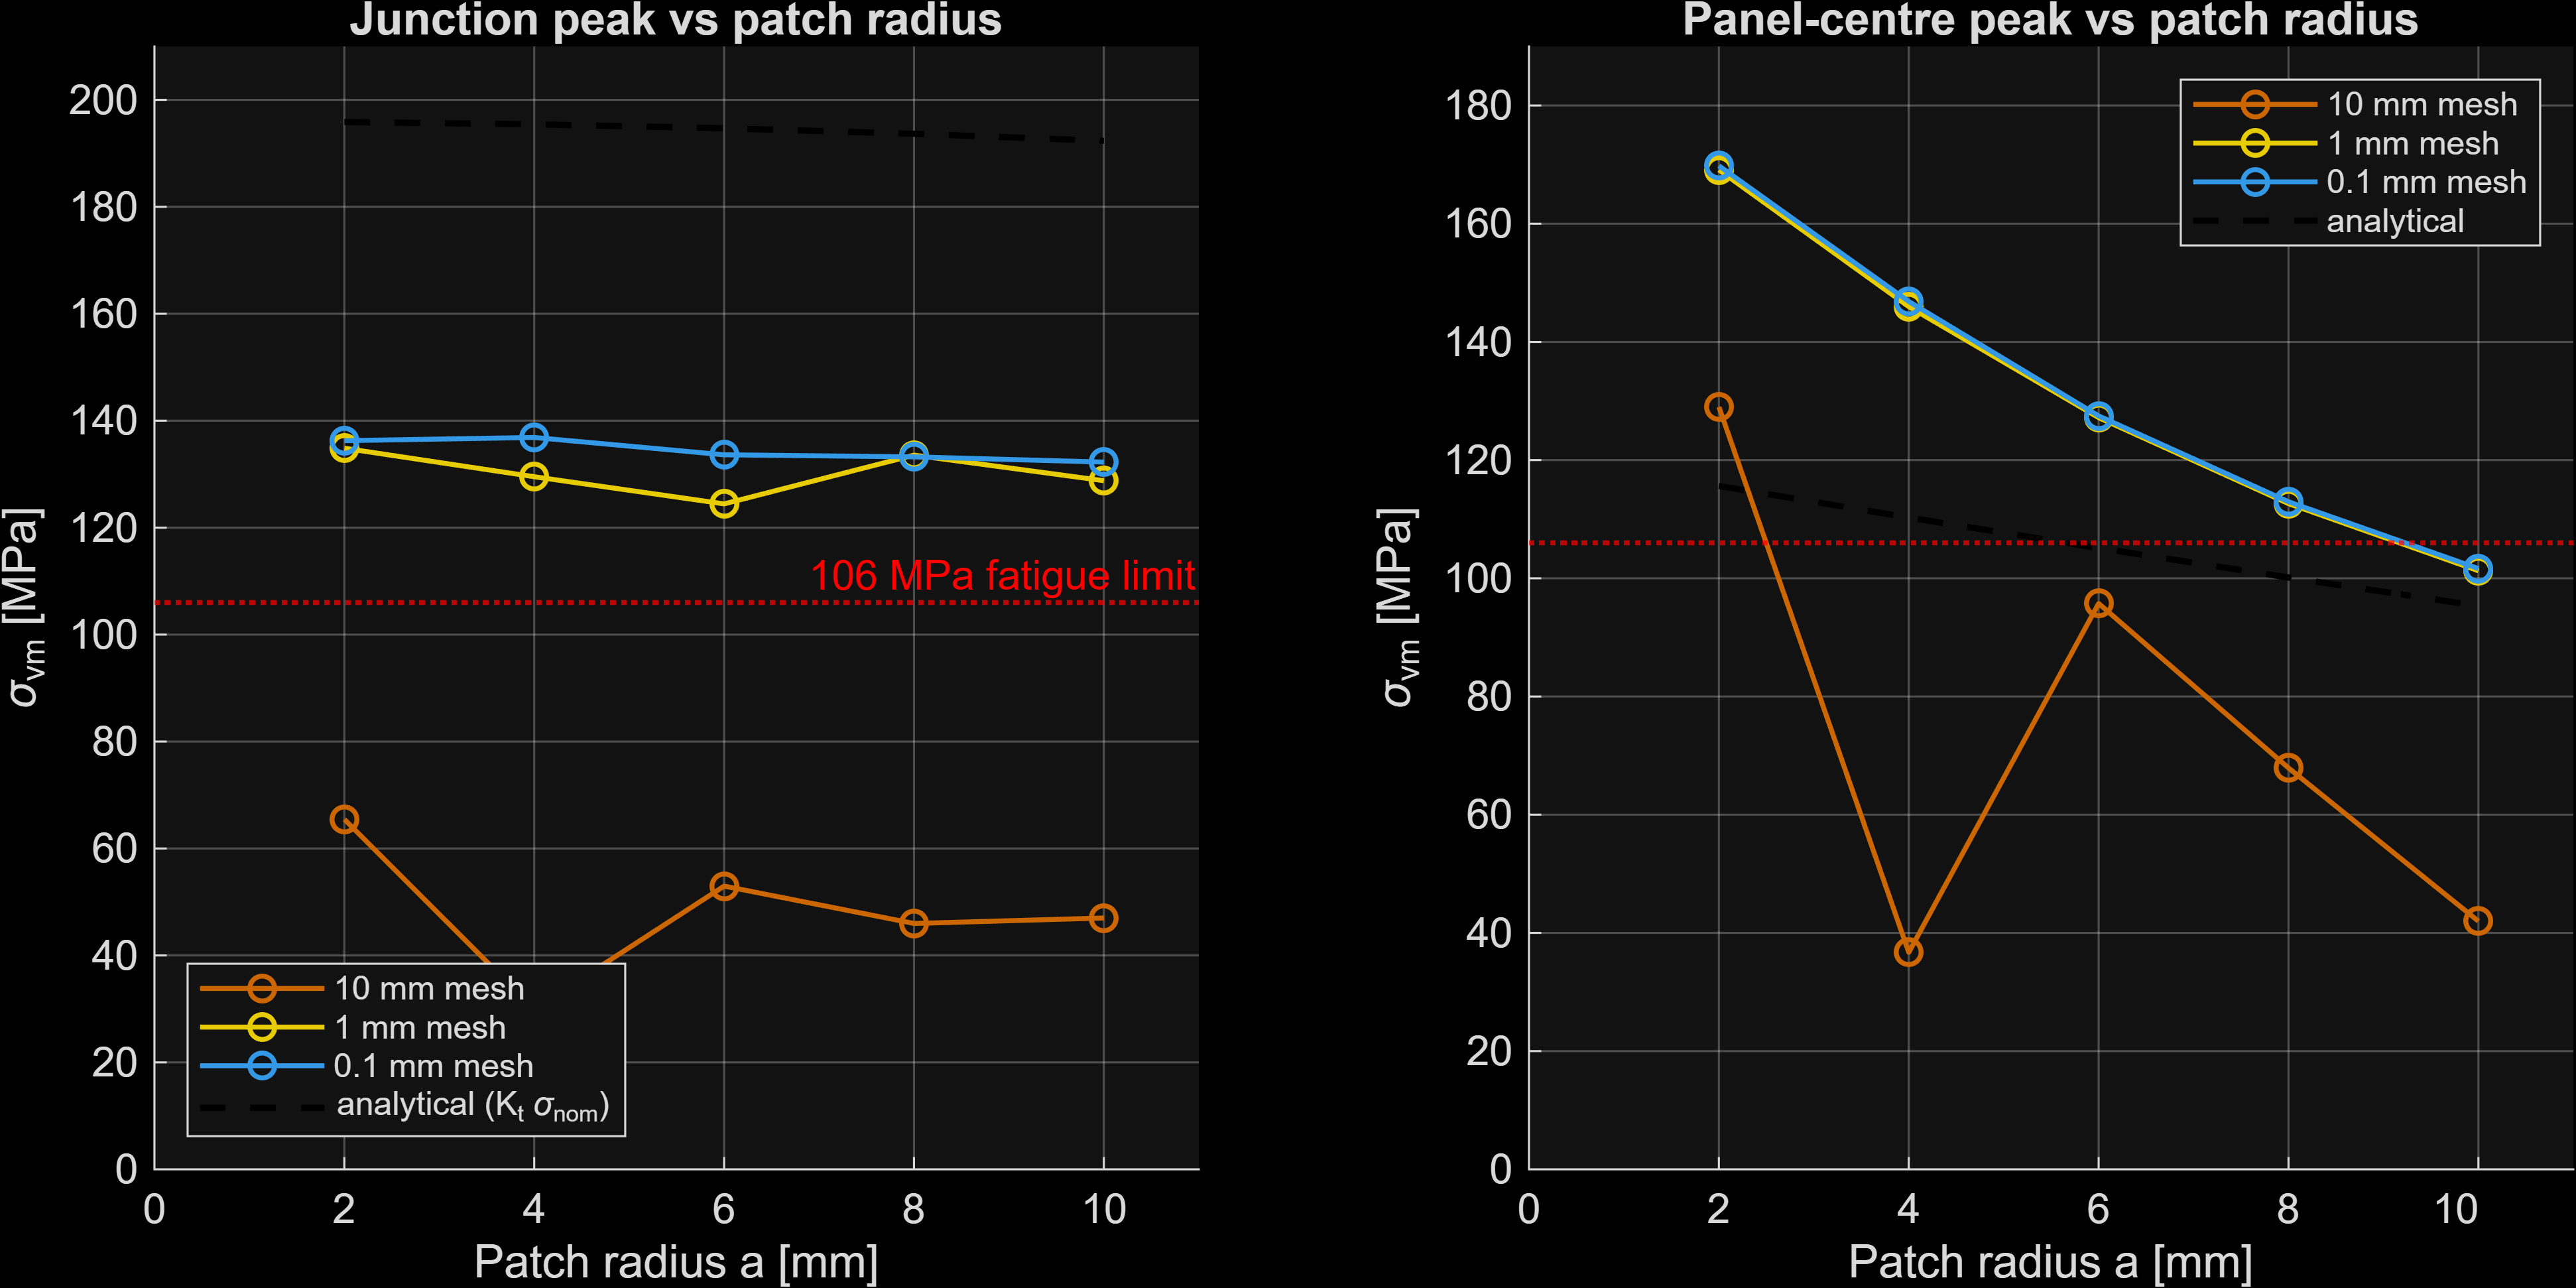
\includegraphics[width=0.8\textwidth]{fea_vs_analytical_comparison.png}
  \caption{FEA junction (left) and centre (right) peaks against patch radius on the three meshes, with the analytical values (dashed) and the \SI{106}{MPa} fatigue limit (dotted), at \SI{400}{N}.}
  \label{fig:peaks}
\end{figure}

\begin{table}[htbp]
  \centering
  \caption{Calibration factors $C = \sigma_\text{FEA}/\sigma_\text{analytical}$ on each mesh. $C_j$ compares with the $K_t$-amplified analytical junction stress.}
  \label{tab:calibmesh}
  \begin{tabular}{rrrrrrr}
    \toprule
    & \multicolumn{3}{c}{$C_j$} & \multicolumn{3}{c}{$C_c$} \\
    \cmidrule(lr){2-4}\cmidrule(lr){5-7}
    $a$ (mm) & \SI{10}{mm} & \SI{1}{mm} & \SI{0.1}{mm} & \SI{10}{mm} & \SI{1}{mm} & \SI{0.1}{mm} \\
    \midrule
    2 & 0.33 & 0.69 & 0.70 & 1.12 & 1.46 & 1.47 \\
    4 & 0.15 & 0.66 & 0.70 & 0.33 & 1.32 & 1.33 \\
    6 & 0.27 & 0.64 & 0.69 & 0.91 & 1.21 & 1.21 \\
    8 & 0.24 & 0.69 & 0.69 & 0.68 & 1.12 & 1.13 \\
    10 & 0.24 & 0.67 & 0.69 & 0.44 & 1.06 & 1.07 \\
    \bottomrule
  \end{tabular}
\end{table}

\begin{table}[htbp]
  \centering
  \caption{FEA against analytical peaks and calibration factors on the converged \SI{0.1}{mm} mesh (\href{\blob/scripts\%20and\%20outputs/tier_1/output/0.1mm_meshing/fea_vs_analytical.csv}{\texttt{0.1mm\_meshing/fea\_vs\_analytical.csv}}). Stresses in MPa at \SI{400}{N}.}
  \label{tab:calib}
  \begin{tabular}{rrrrrrr}
    \toprule
    $a$ (mm) & FEA $j$ & Analytical $j$ & $C_j$ & FEA $c$ & Analytical $c$ & $C_c$ \\
    \midrule
    2 & 136.3 & 195.9 & 0.70 & 169.8 & 115.6 & 1.47 \\
    4 & 136.9 & 195.4 & 0.70 & 146.8 & 110.3 & 1.33 \\
    6 & 133.6 & 194.7 & 0.69 & 127.5 & 105.1 & 1.21 \\
    8 & 133.2 & 193.7 & 0.69 & 113.0 & 100.1 & 1.13 \\
    10 & 132.3 & 192.3 & 0.69 & 101.6 & 95.3 & 1.07 \\
    \bottomrule
  \end{tabular}
\end{table}

\begin{figure}[htbp]
  \centering
  \begin{subfigure}[b]{0.32\textwidth}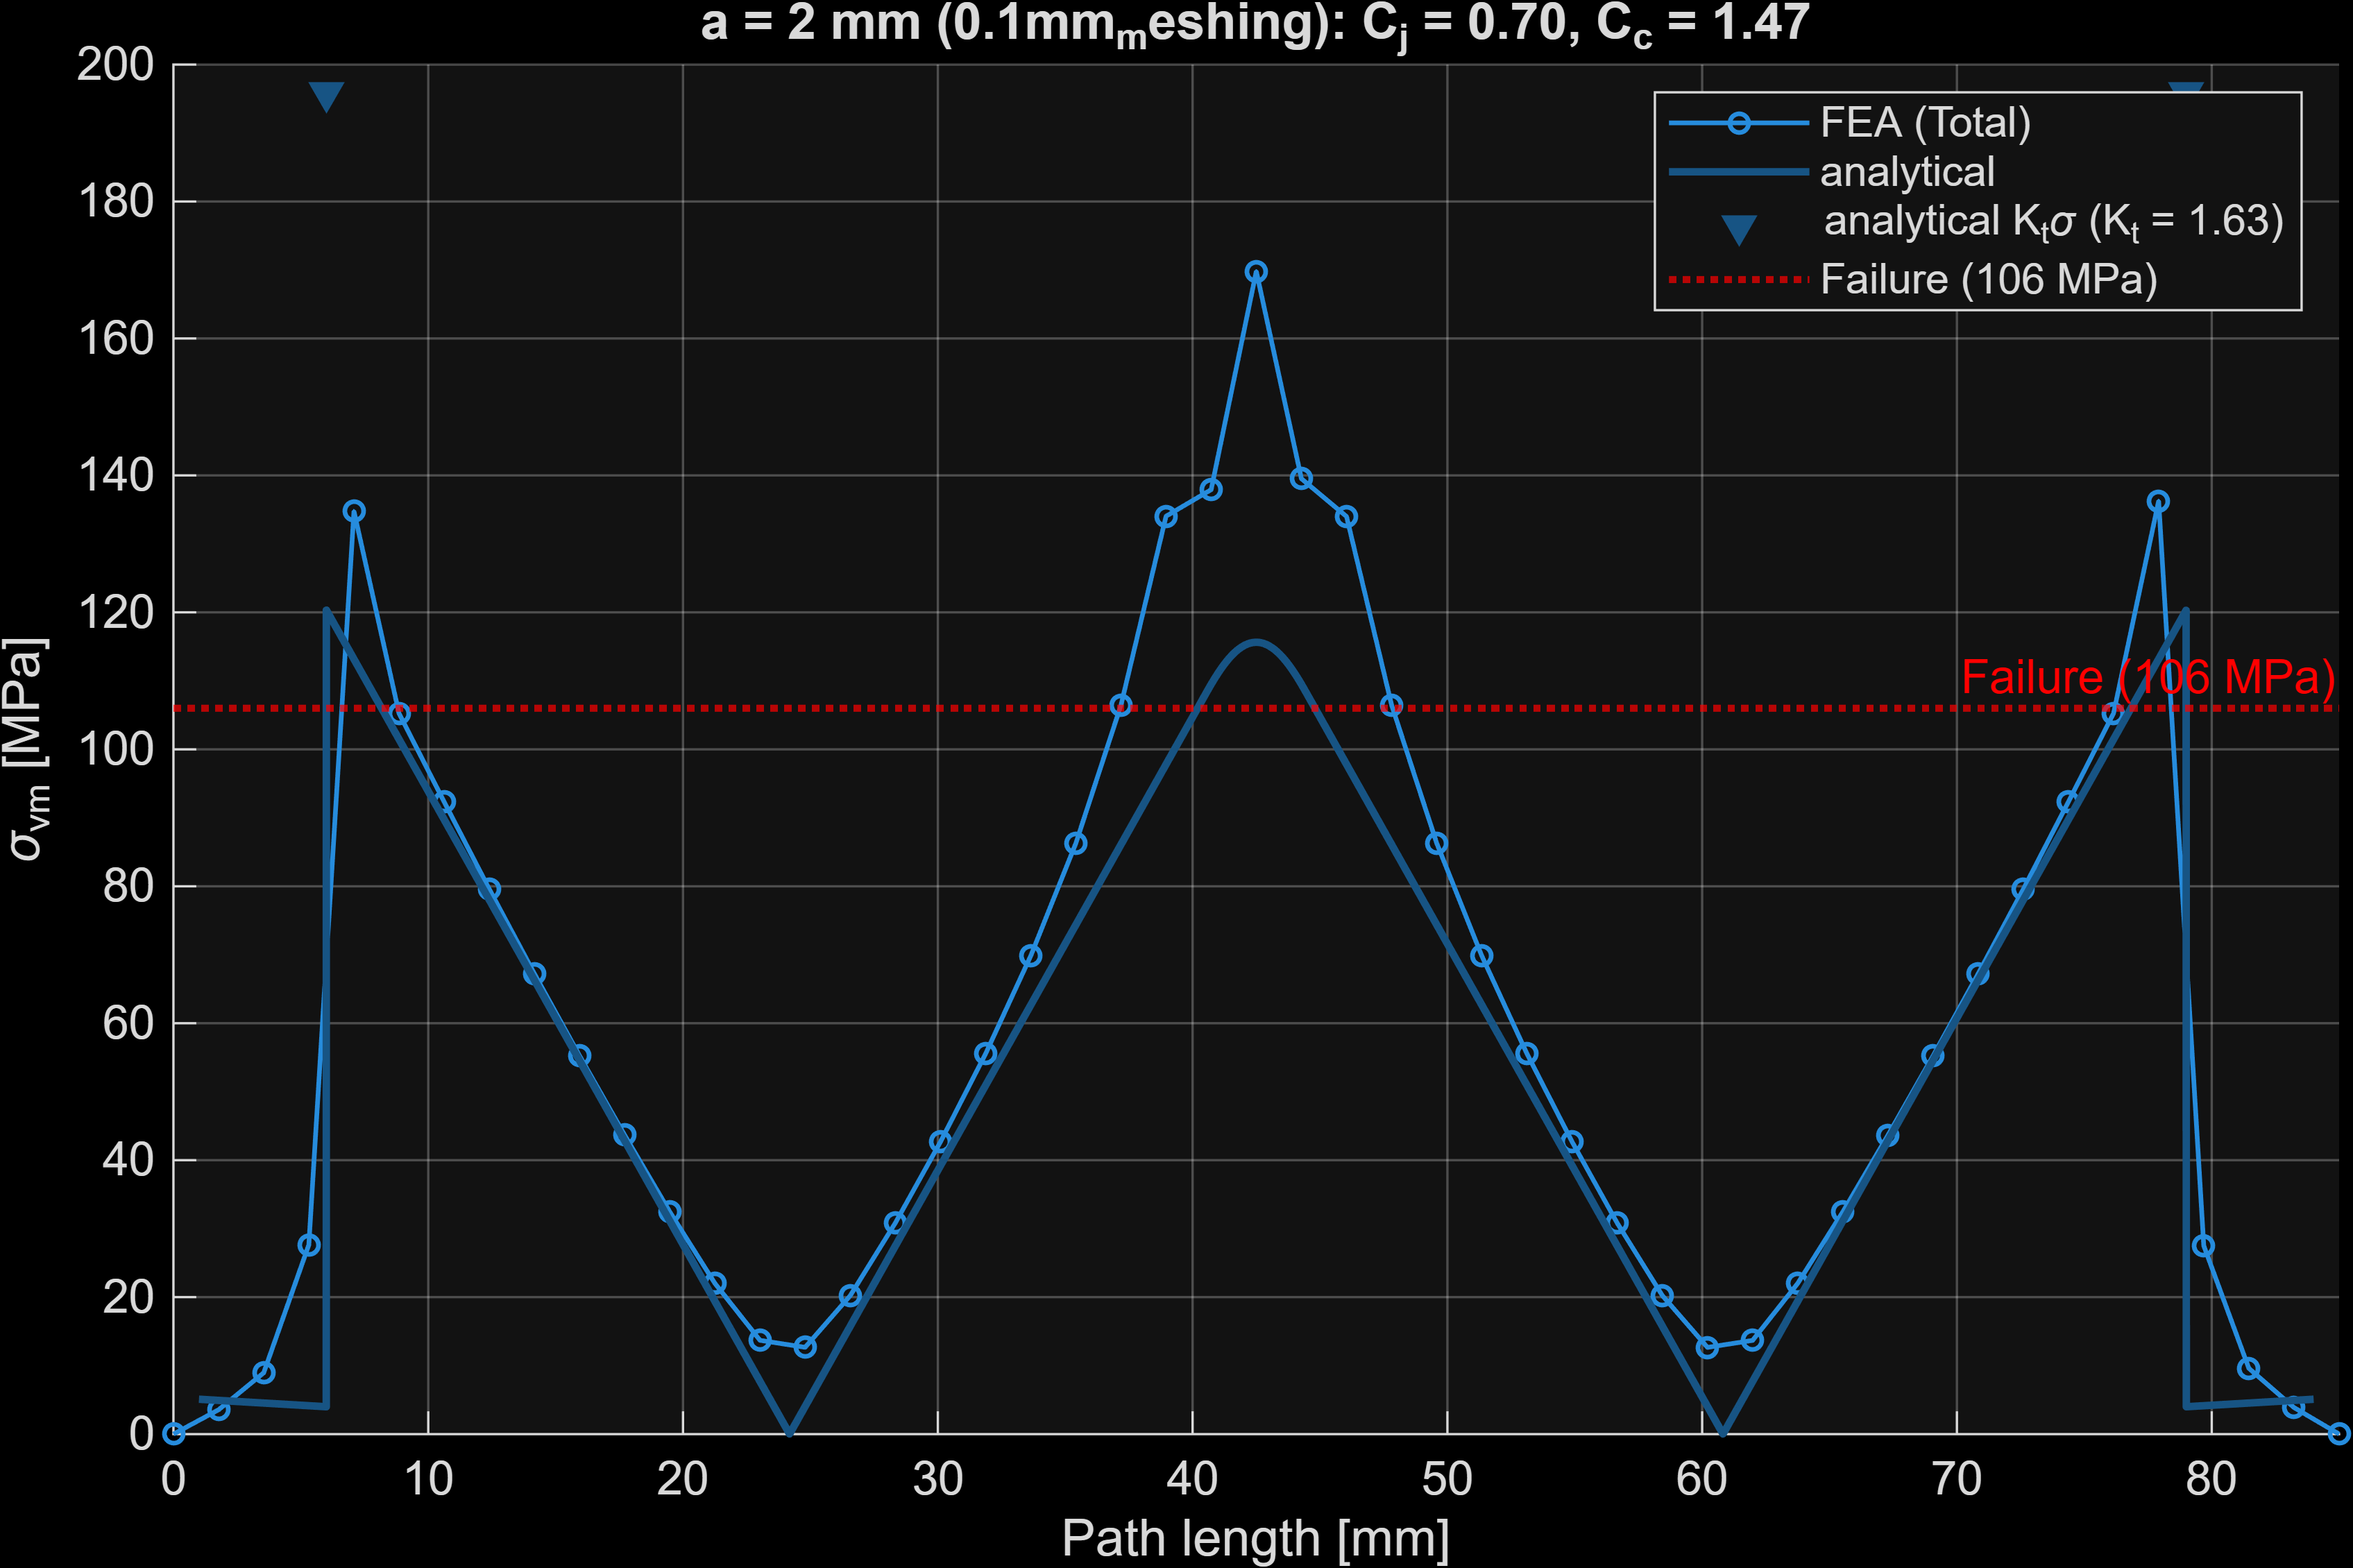
\includegraphics[width=\linewidth]{0.1mm_meshing/overlay_a2.png}\caption{$a = 2$}\end{subfigure}\hfill
  \begin{subfigure}[b]{0.32\textwidth}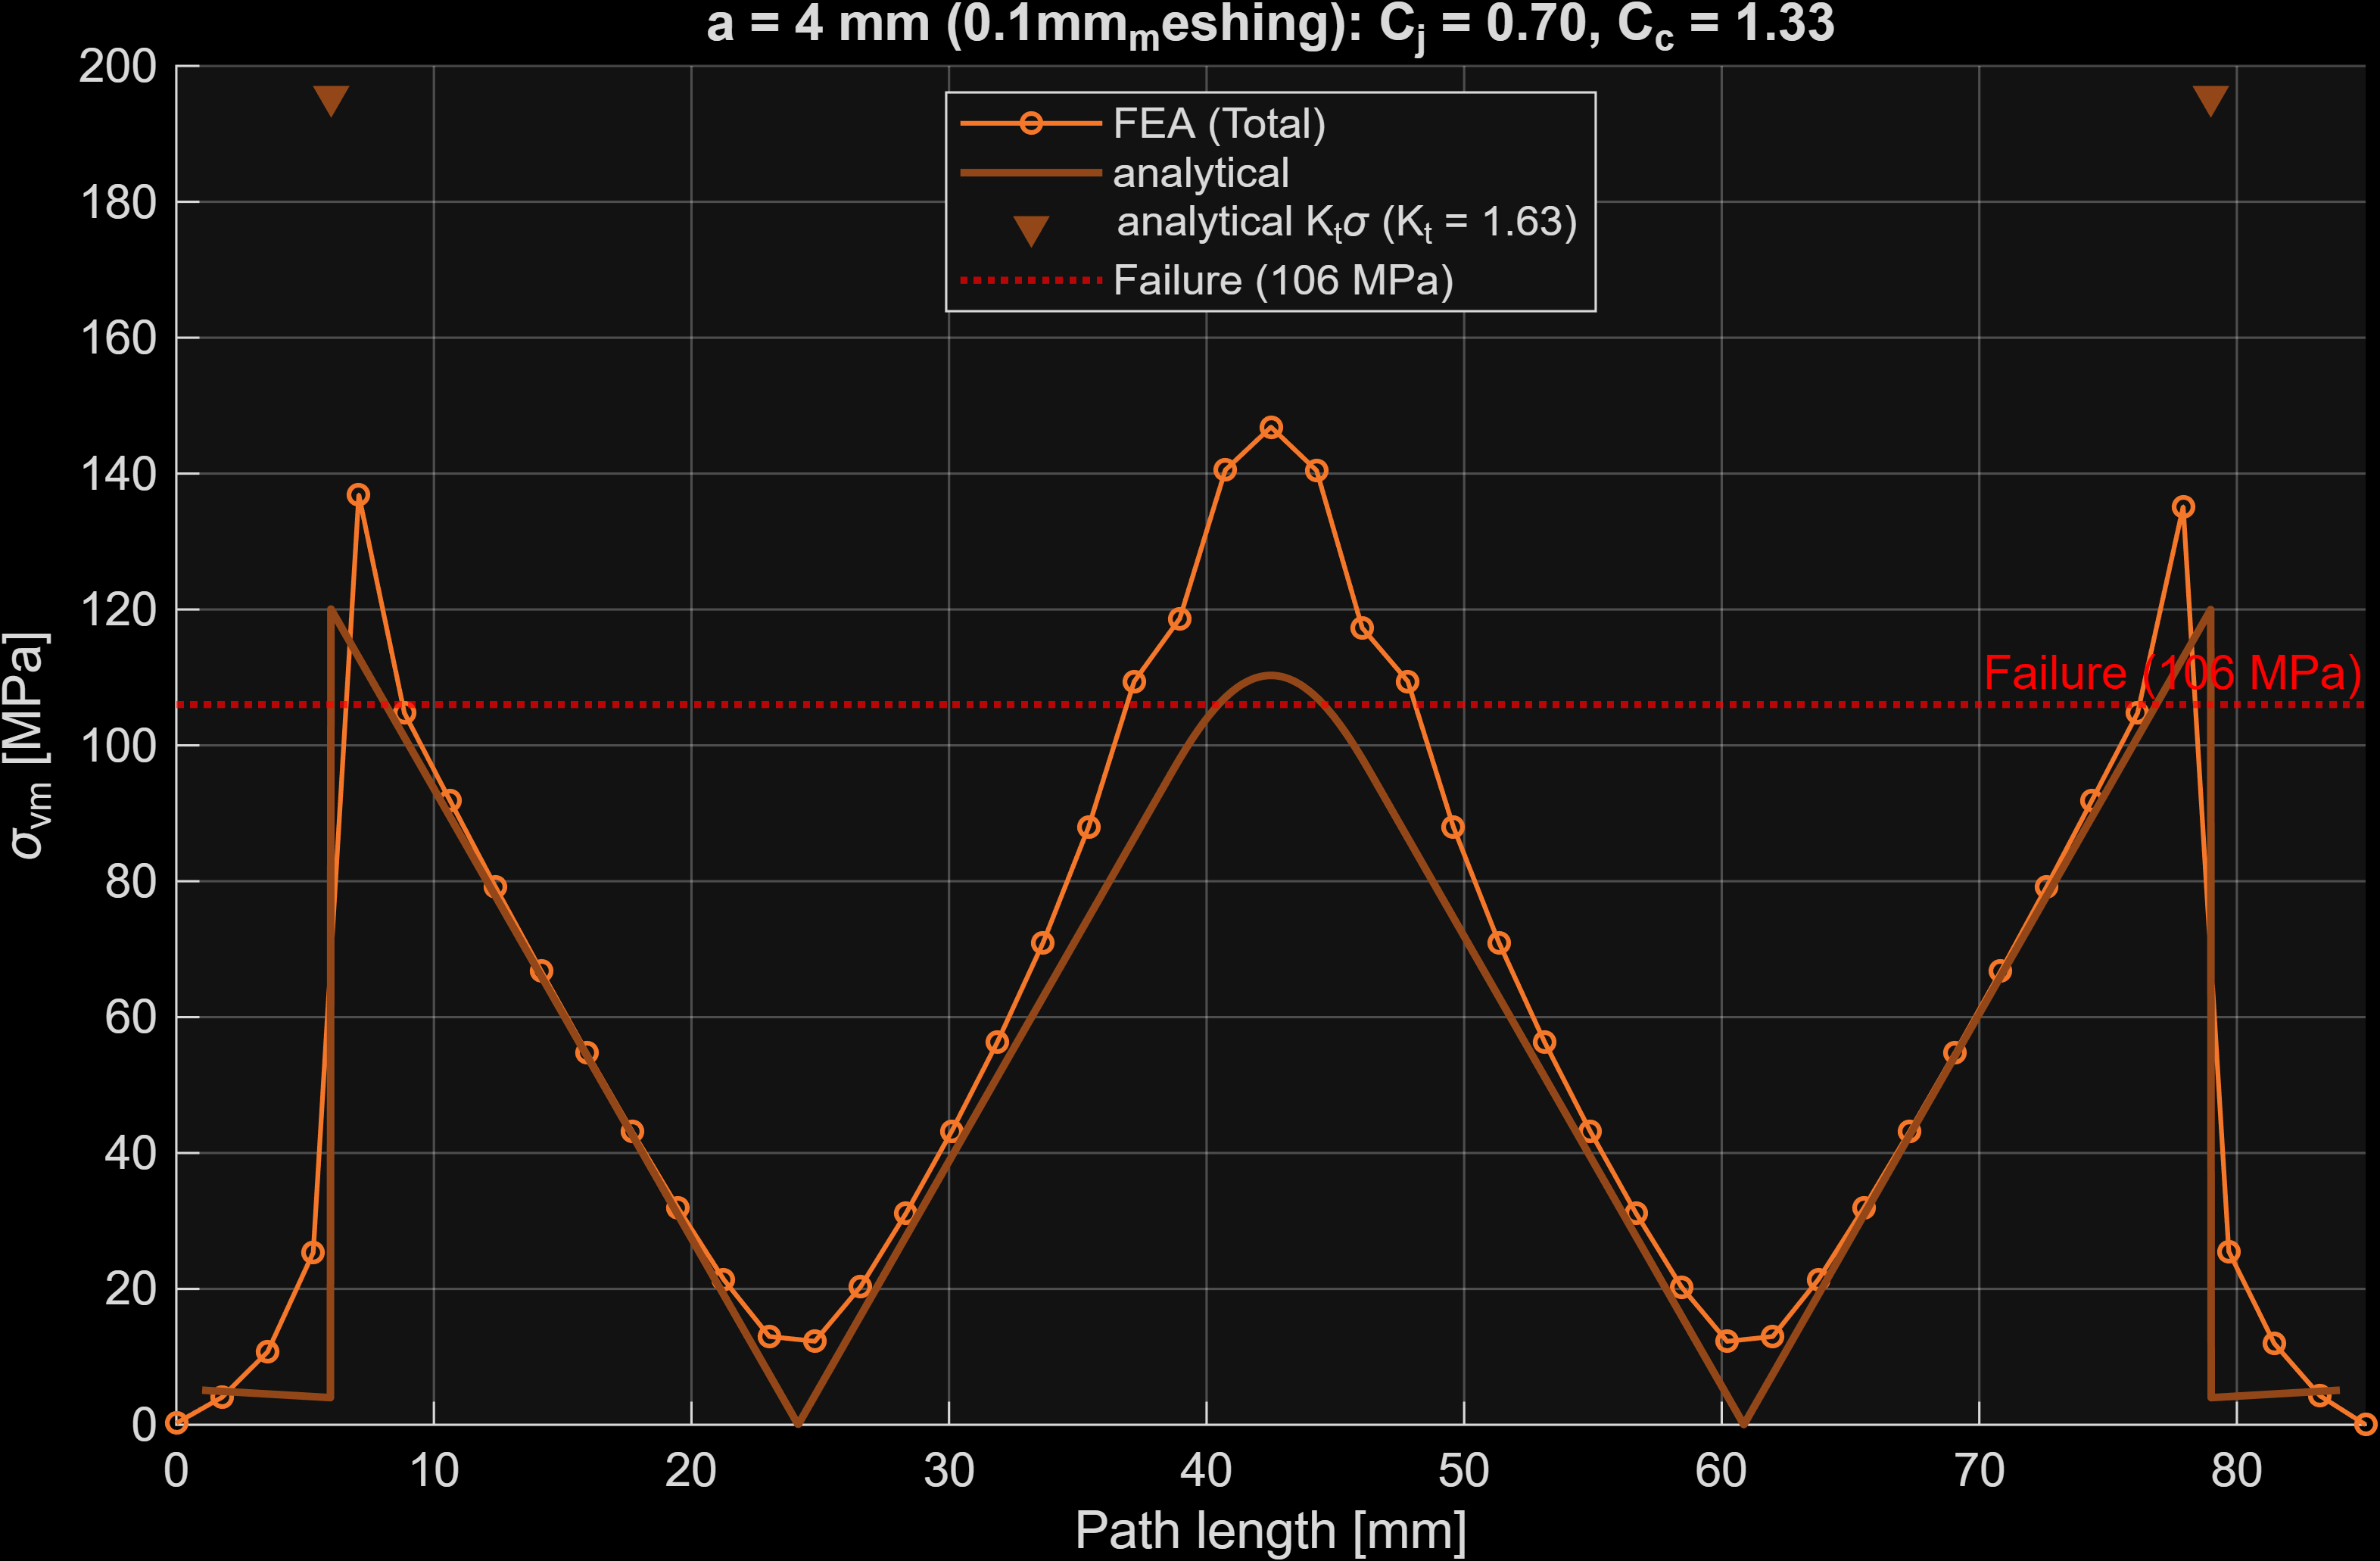
\includegraphics[width=\linewidth]{0.1mm_meshing/overlay_a4.png}\caption{$a = 4$}\end{subfigure}\hfill
  \begin{subfigure}[b]{0.32\textwidth}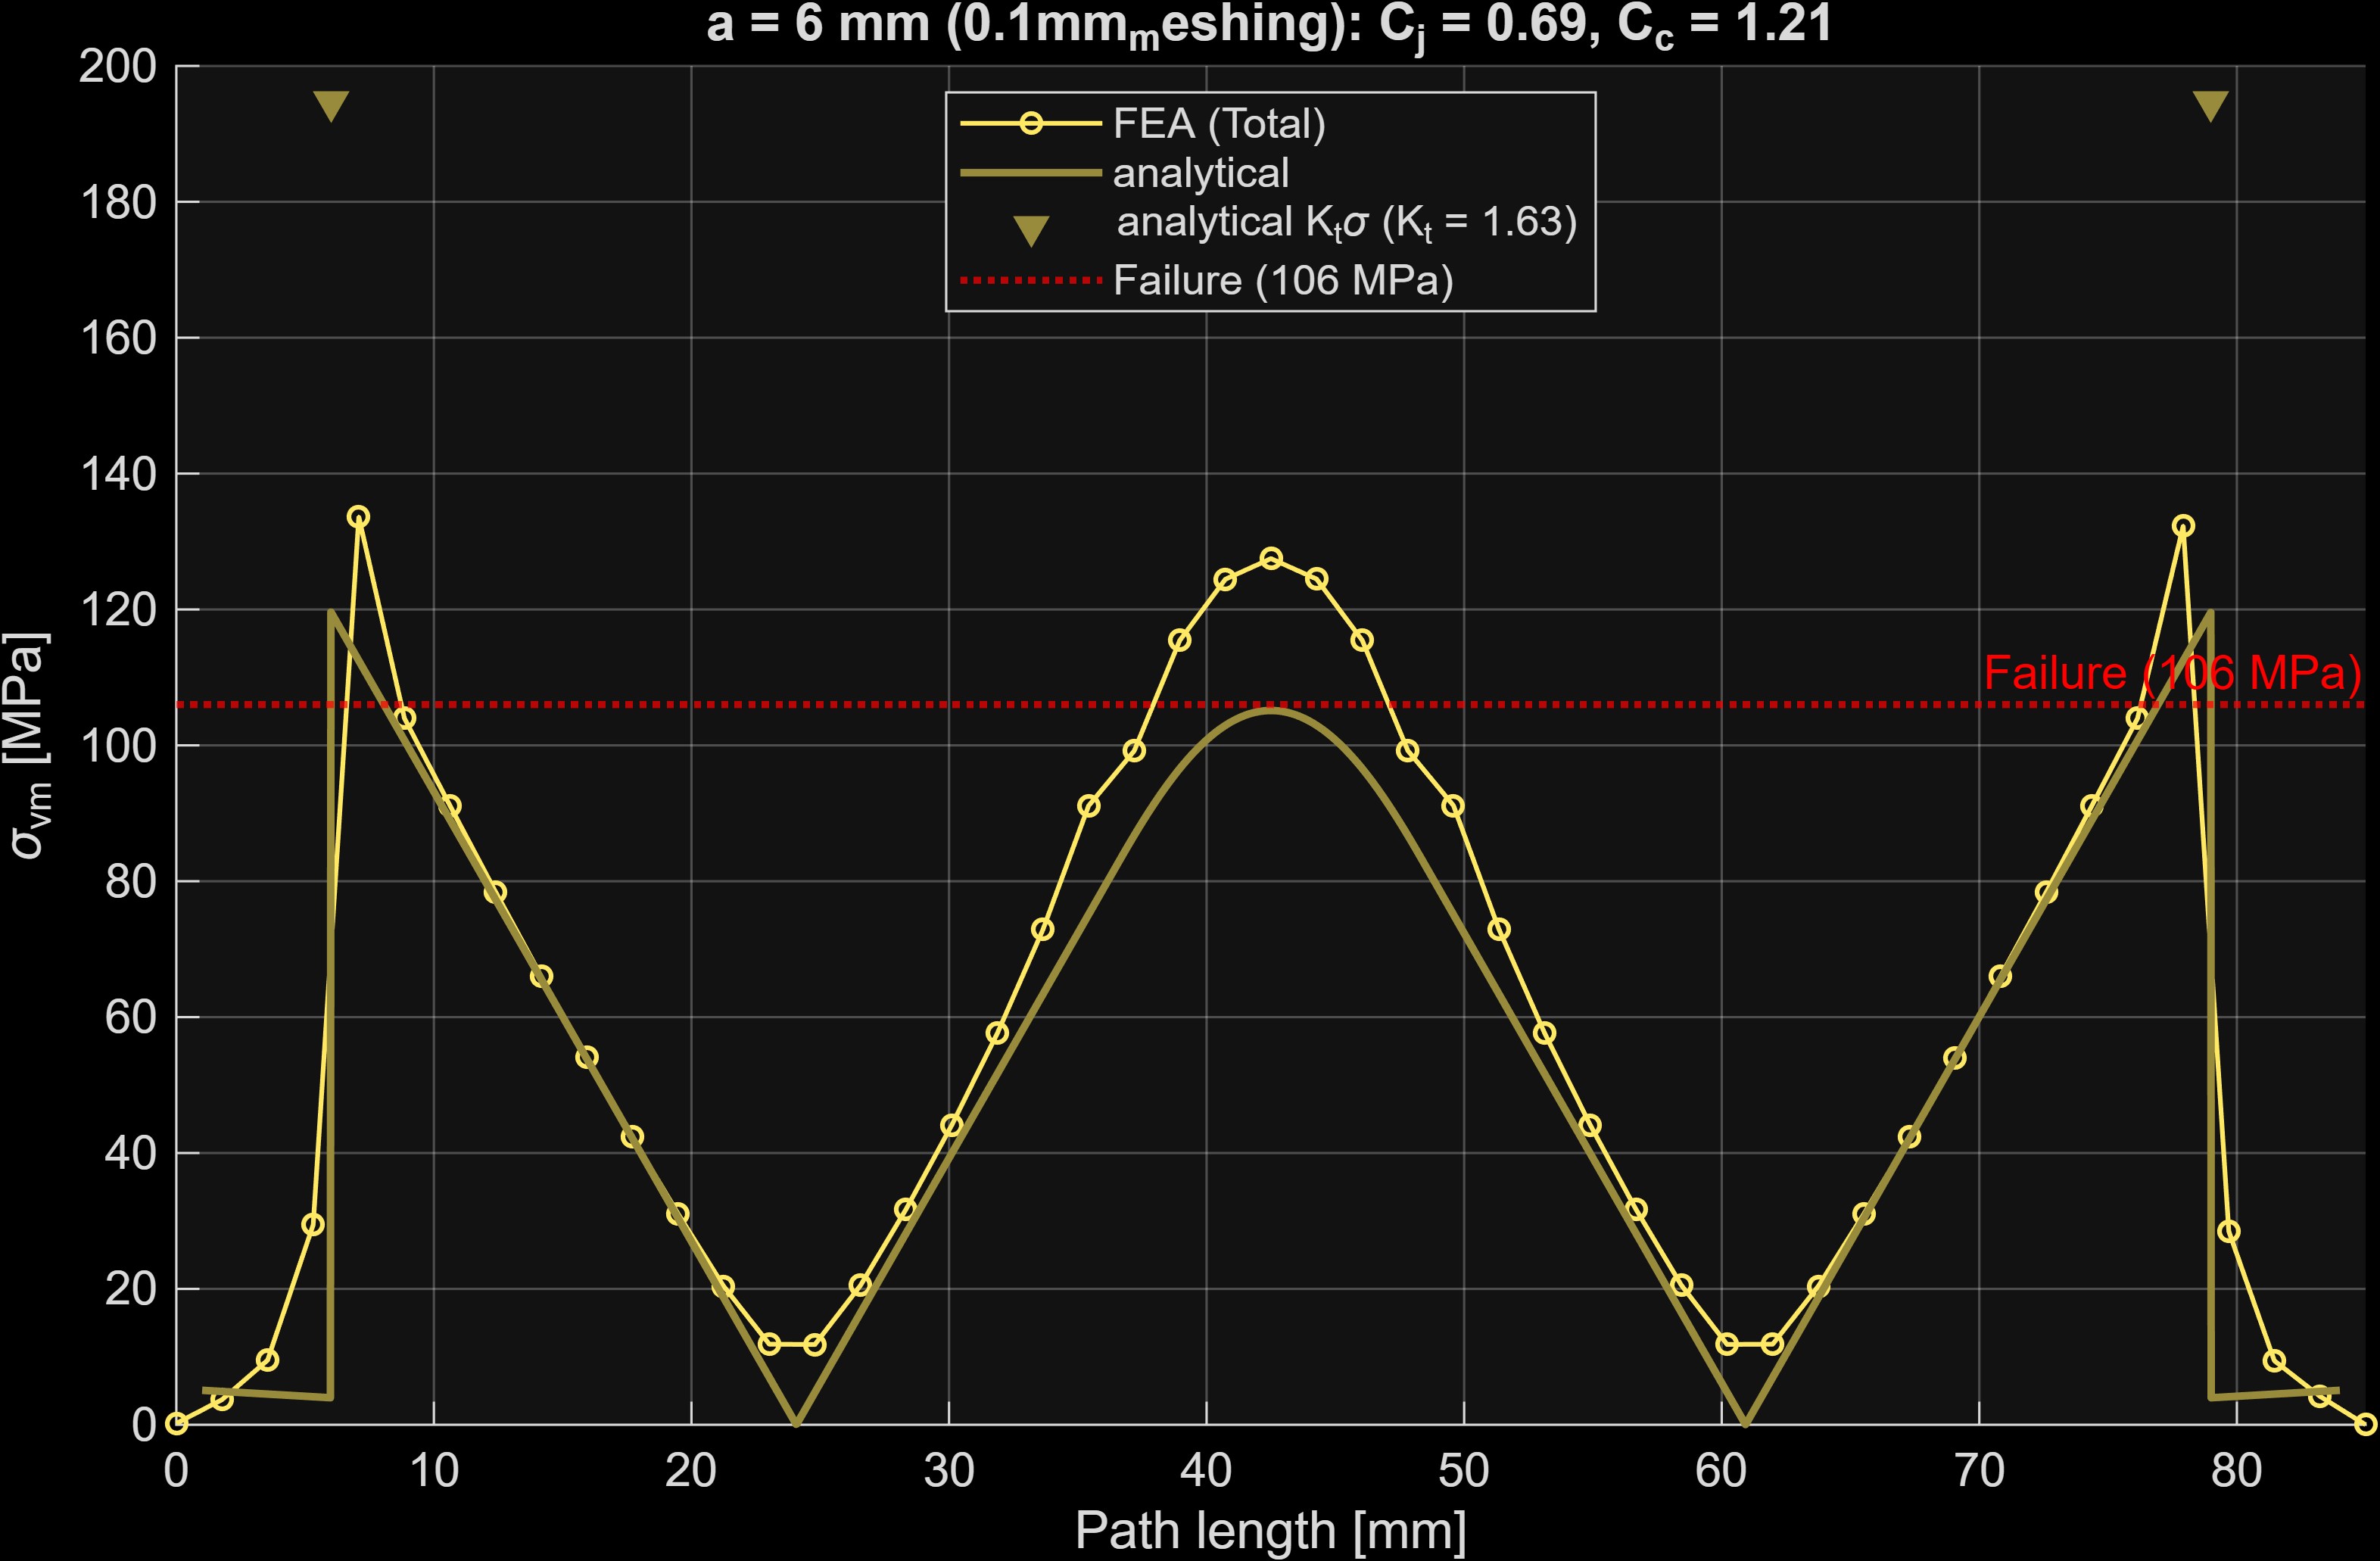
\includegraphics[width=\linewidth]{0.1mm_meshing/overlay_a6.png}\caption{$a = 6$}\end{subfigure}\\[4pt]
  \begin{subfigure}[b]{0.32\textwidth}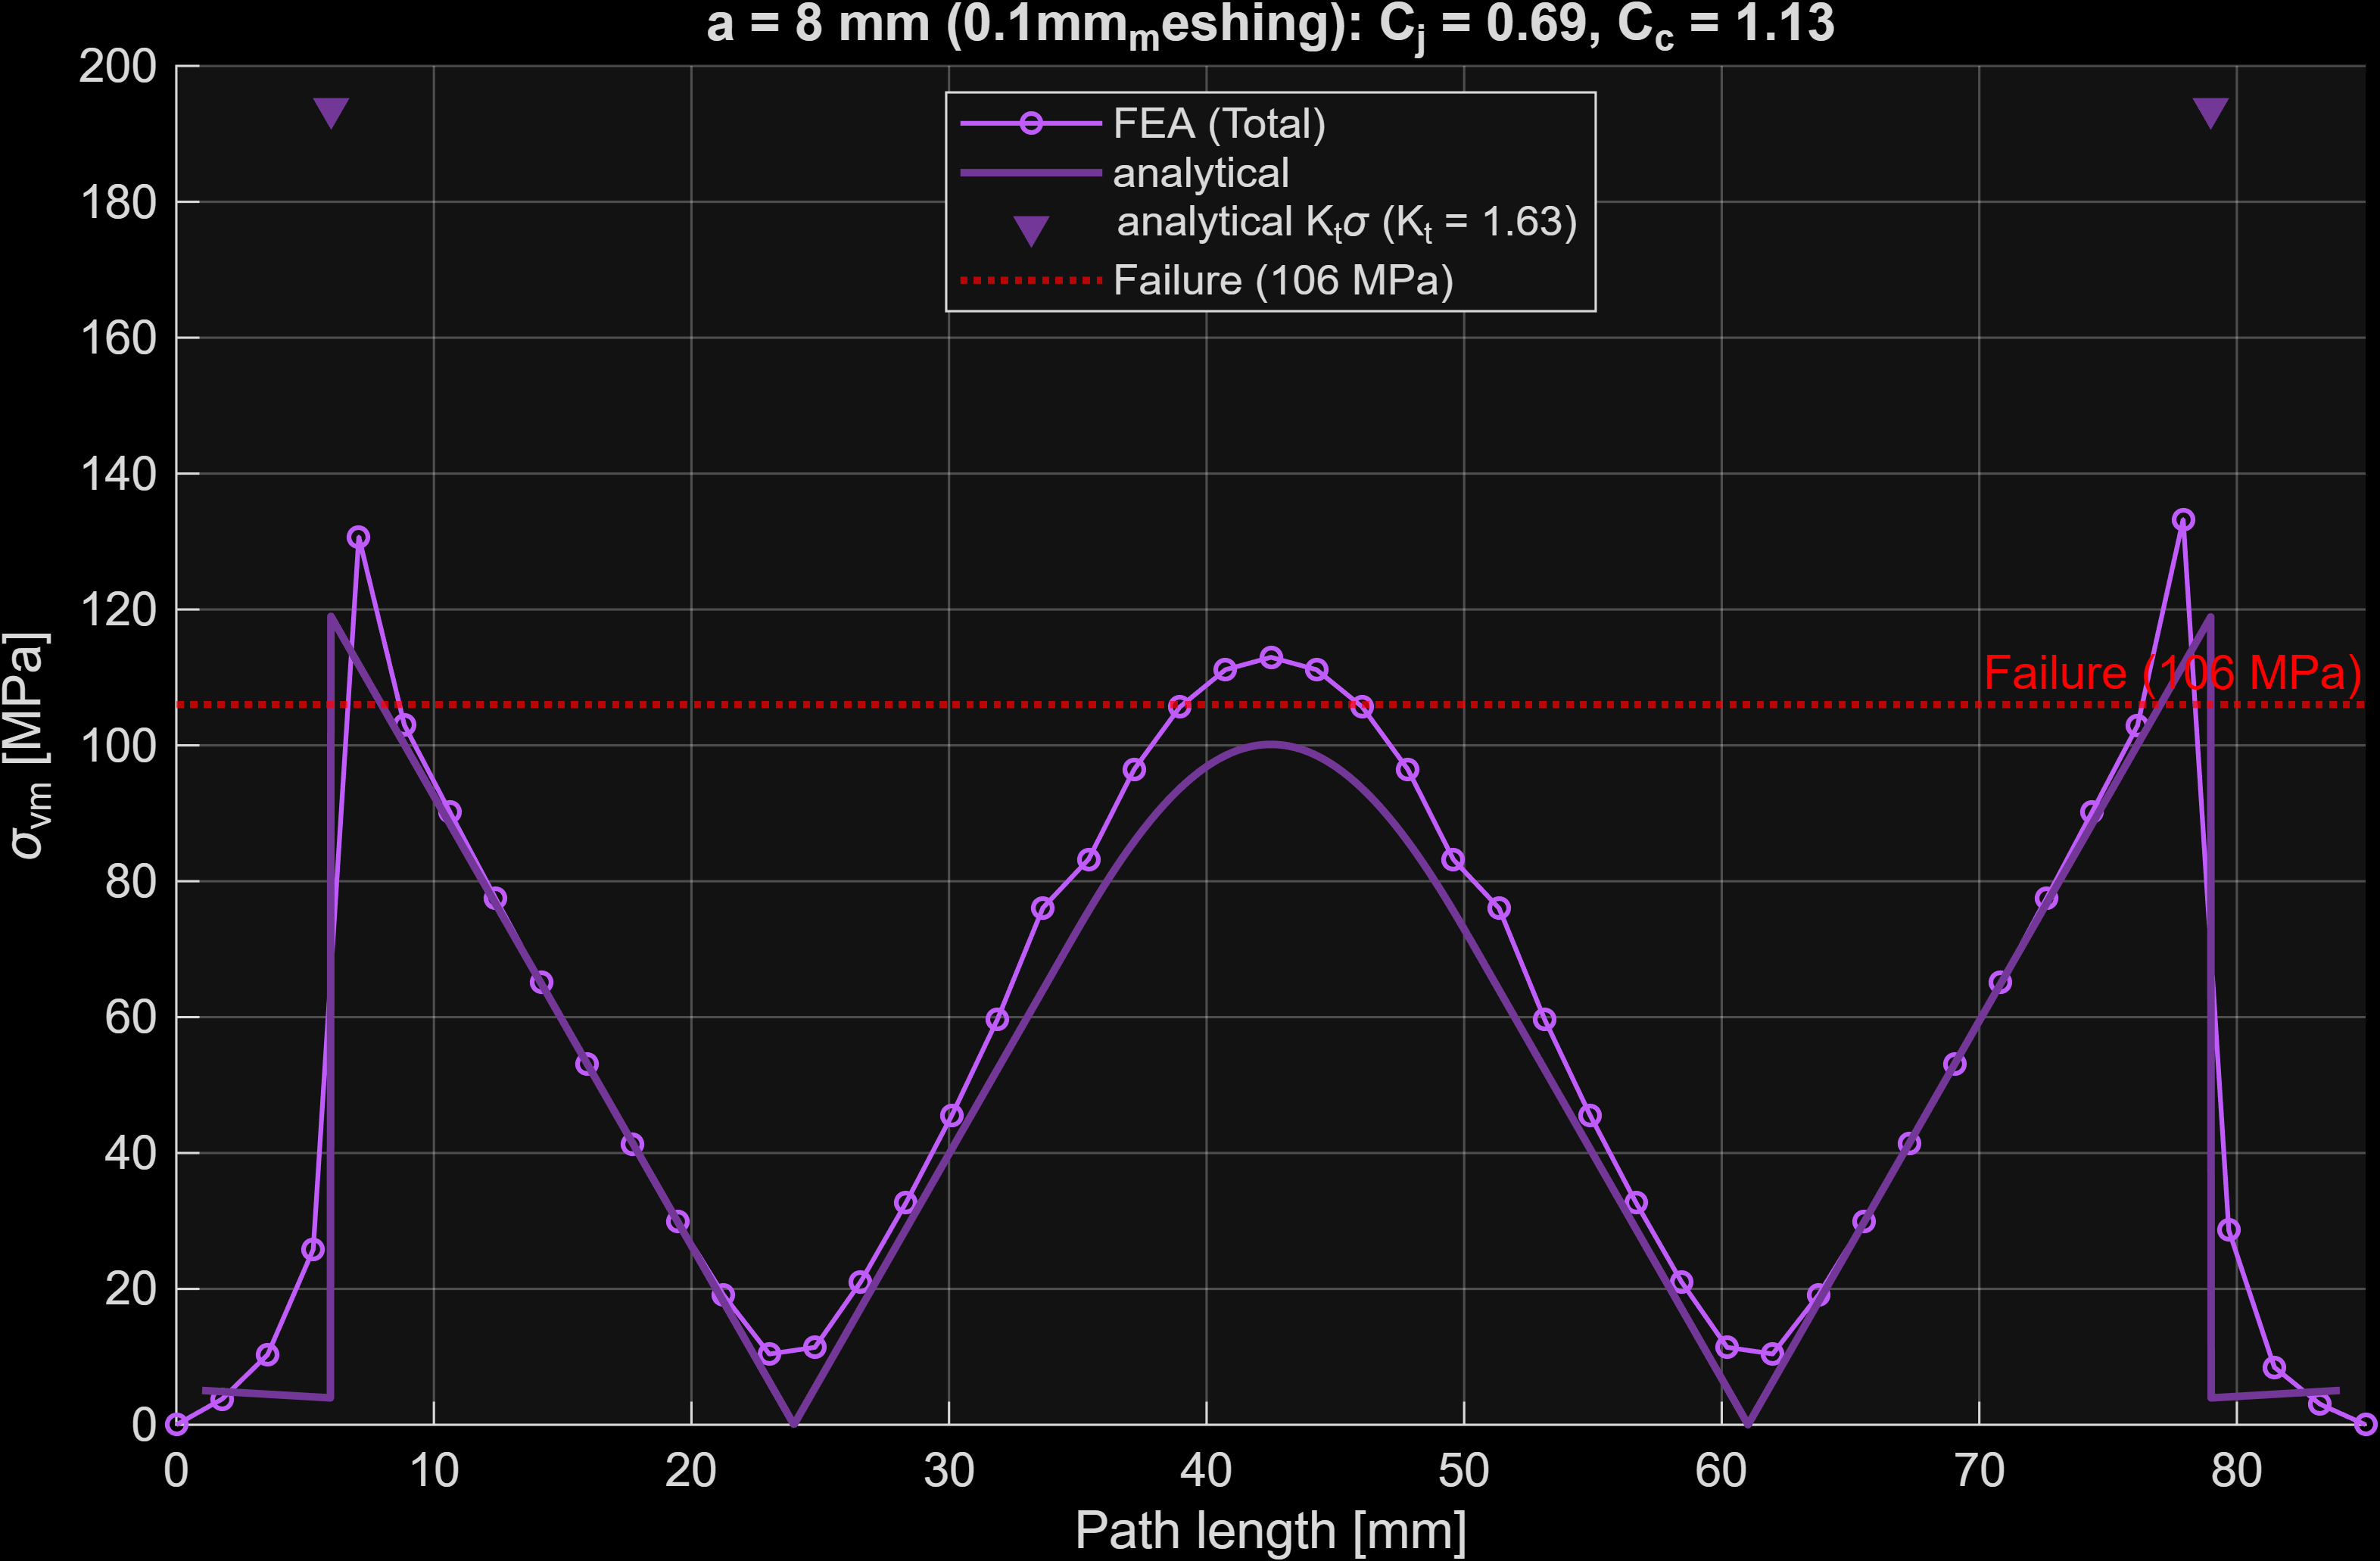
\includegraphics[width=\linewidth]{0.1mm_meshing/overlay_a8.png}\caption{$a = 8$}\end{subfigure}\hspace{0.02\textwidth}
  \begin{subfigure}[b]{0.32\textwidth}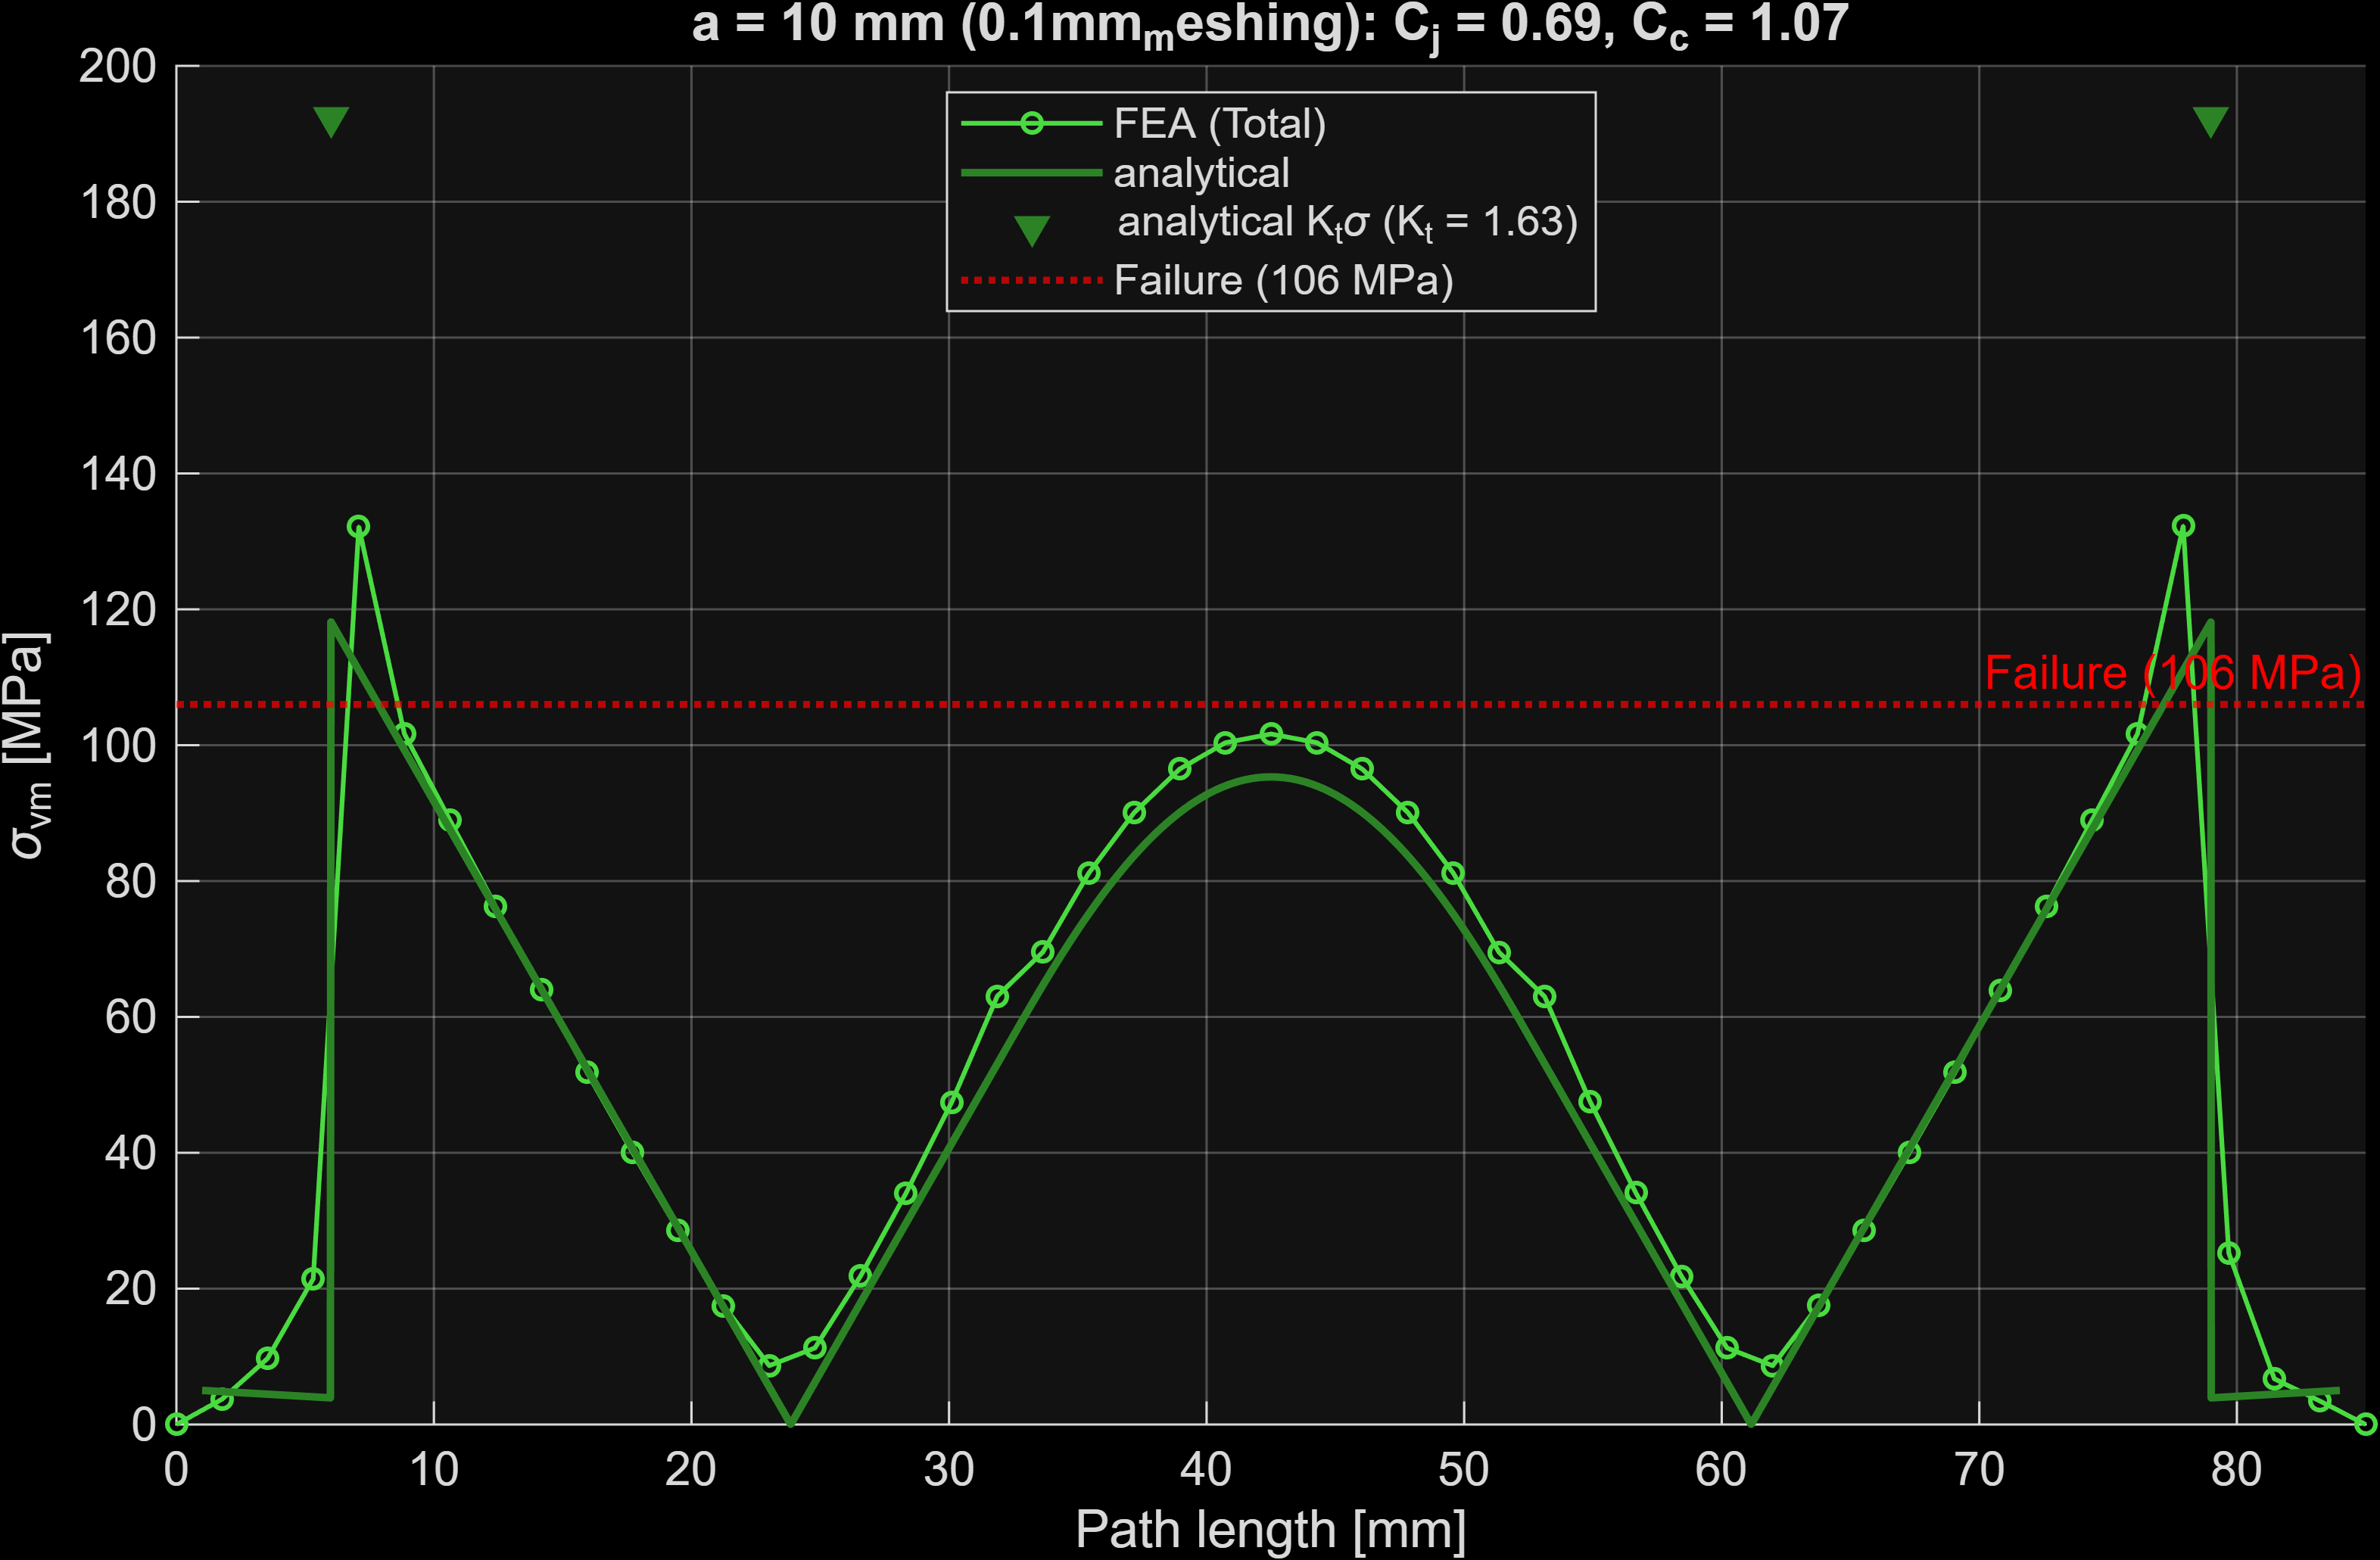
\includegraphics[width=\linewidth]{0.1mm_meshing/overlay_a10.png}\caption{$a = 10$}\end{subfigure}
  \caption{FEA (markers) and analytical (solid) $\sigma_\text{vm}$ along the path for each patch radius (mm) on the converged \SI{0.1}{mm} mesh, at \SI{400}{N}.}
  \label{fig:overlays}
\end{figure}


% ---------------------------------------------------------------
\section{Discussion}

\paragraph{Mesh convergence.}
The \SI{10}{mm} results are an artefact of the mesh, not of the physics. The elements are five times the skin thickness and larger than the patch diameter for $a \le \SI{4}{mm}$, so the patch pressure and the through-thickness bending gradient are not resolved, and how the patch face happens to fall on the mesh decides the answer. That is the most likely origin of the non-monotonic $a = \SI{4}{mm}$ result on the coarse mesh ($C_c = 0.33$): on the \SI{1}{mm} and \SI{0.1}{mm} meshes it becomes $C_c = 1.32$ and $1.33$ and sits in its proper place between $a = 2$ and $6$\,mm. The \SI{1}{mm} mesh is adequate for the panel centre, but its junction values are still up to \SI{7}{\percent} below the \SI{0.1}{mm} ones, so the \SI{0.1}{mm} mesh is used for everything below.

\paragraph{Panel centre.}
On the converged mesh the beam model under-predicts the centre stress at every radius, by \SI{32}{\percent} at $a = \SI{2}{mm}$ ($C_c = 1.47$), falling steadily to \SI{6}{\percent} at $a = \SI{10}{mm}$ ($C_c = 1.07$). The direction is the one expected: the beam spreads the load over the full \SI{40}{mm} width, while the real plate carries it more locally, and the effect is strongest for the sharpest contact. As $a$ grows the FEA centre stress still falls faster than the beam predicts (\SI{170}{MPa} to \SI{102}{MPa}, a drop of \SI{40}{\percent}, against \SI{116}{MPa} to \SI{95}{MPa}, \SI{18}{\percent}), which is the plate effect again: a wide patch is shared in two directions, which a one-dimensional strip cannot capture. Away from the patch the FEA follows the analytical slopes closely (Figure~\ref{fig:overlays}). Because the beam is \emph{non-conservative} at the centre, a design check based on it alone would under-estimate the stress under a sharp rock.

\paragraph{Junction.}
The $K_t$-amplified analytical junction stress is about 1.45 times the converged FEA value ($C_j = 0.69$--$0.70$, almost independent of $a$ and of the mesh once it is at or below \SI{1}{mm}). On the unconverged \SI{10}{mm} mesh the discrepancy would appear to be a factor of three to six; that is largely a mesh artefact. A more telling comparison is with the plain beam stress before $K_t$: the FEA junction peaks are $1.12$--$1.14$ times the nominal von Mises stress of 118--\SI{120}{MPa}, i.e.\ the FEA behaves as if the effective concentration factor on the sampled path were about 1.1, not 1.63. This has two consequences. First, the rigid-clamp and width-averaging simplifications cannot be large sources of error, because the FEA junction stress is slightly \emph{above} the beam moment's nominal value rather than relieved below it, so the converged data do not support them as explanations of the discrepancy. Second, the discrepancy sits almost entirely in $K_t$. The most likely reasons are that Peterson's chart is for a symmetric shoulder, which is more severe than the one-sided T-junction here, and that the FEA path samples every \SI{1.77}{mm} and so may step over the true local peak of the \SI{1}{mm} fillet. The second point means the FEA junction values may be a lower bound of the real peak; the sharp spike at $S \approx \SI{7}{mm}$ is a single sample on every curve.

\paragraph{Implications.}
At \SI{400}{N} both critical locations exceed the \SI{106}{MPa} fatigue limit for sharp rocks. The FEA junction stress (132--\SI{137}{MPa}) is above the limit for every patch size studied. The centre stress governs for $a \le \SI{4}{mm}$ (\SI{170}{MPa} and \SI{147}{MPa}, against 136--\SI{137}{MPa} at the junction), is still above the limit at $a = 6$ and \SI{8}{mm} (\SI{127}{MPa}, \SI{113}{MPa}) but is then lower than the junction, and falls just below the limit at $a = \SI{10}{mm}$ (\SI{102}{MPa}). Cracks would therefore be expected to start at the centre before the junction only for sharp rocks ($a \le \SI{4}{mm}$; the crossover lies between 4 and \SI{6}{mm}); for blunter rocks the junction is the more likely initiation site, which is consistent with the service damage reported where the skin meets the grousers.

% ---------------------------------------------------------------
\section{Conclusions}

The thin skin of the wheel is weakest where a hard rock presses on it. A rock pressing on the skin between two grousers bends it like a clamped strip, and that bending concentrates stress in two places: directly under the rock, and at the corner where the skin joins the thick grouser. For the load studied, the stress at the corner is above the fatigue limit of the aluminium for every rock size tested, and the stress under the rock is above it too when the rock is sharp. Repeated passes over such rocks can therefore start cracks at either place. Sharper rocks are the more dangerous under the patch, while for blunter rocks the corner is the more likely starting point. This matches where cracks have actually been reported on the wheels. A simple hand calculation shows the same overall pattern and is good for quick estimates, but it under-estimates the stress under sharp rocks and over-estimates it at the corner, so it should be corrected using the simulation before it is trusted for design. The mesh study showed that the simulation is only trustworthy when the model is divided finely enough: the coarsest mesh gave wrong answers, while the two finer ones agree closely.

% ---------------------------------------------------------------
\FloatBarrier
\section*{Repository resources}
\begin{itemize}\raggedright\setlength\itemsep{0pt}
  \item Analytical model: \href{\blob/scripts\%20and\%20outputs/tier_1/path_stress_analytical.m}{\texttt{scripts and outputs/tier\_1/path\_stress\_analytical.m}}
  \item FEA comparison (loops over all three meshes): \href{\blob/scripts\%20and\%20outputs/tier_1/fea_vs_analytical.m}{\texttt{scripts and outputs/tier\_1/fea\_vs\_analytical.m}}
  \item Output figures and tables (with README): \href{\tree/scripts\%20and\%20outputs/tier_1/output}{\texttt{scripts and outputs/tier\_1/output}}, with one sub-folder per mesh (\texttt{10mm\_meshing}, \texttt{1mm\_meshing}, \texttt{0.1mm\_meshing})
  \item FEA path data: \href{\tree/Simulation\%20results/Tier\%201}{\texttt{Simulation results/Tier 1}}, one sub-folder per mesh
  \item CAD models: \href{\tree/CAD_models/Tier\%201}{\texttt{CAD\_models/Tier 1}}
  \item Ansys Workbench template used for the simulations: \texttt{Failure\_Analysis\_template\_files} (with its project file \texttt{Failure\_Analysis\_template.wbpj}), in \texttt{Ansys simulation template}
  \item Images used in this report: \href{\tree/media}{\texttt{media}}
\end{itemize}

\begin{thebibliography}{9}
  \bibitem{nasa} NASA Jet Propulsion Laboratory, Mars Science Laboratory (Curiosity) mission reports and status updates on wheel wear. \url{https://mars.nasa.gov/msl/}
  \bibitem{ansys} Ansys Inc., \emph{Ansys Mechanical User's Guide, Release 2025 R1}: Linearized Stress.
  \bibitem{repo} Project repository, \href{\repo}{\texttt{github.com/Shass27/curiosity-perseverance-wheel-fea}}
\end{thebibliography}

\end{document}
